%----------------------------------------------------------------------
% Document class
%----------------------------------------------------------------------
\documentclass[latexfonts,mas]{oru-thesis}

%What to include (useful if you want to send certain portions for review).
%\includeonly{
%  title,
%  abstract,
%  acknowledgements,
%  contents,
%  ch1,
%  ch2,
%  0_backmatter
%}
%----------------------------------------------------------------------


%----------------------------------------------------------------------
% Packages and macros
%----------------------------------------------------------------------

%This needs to be before epsfig
%\usepackage[dvips]{graphicx}
%\usepackage{graphicx}
\usepackage{psfrag}

\usepackage{longtable}
\usepackage{listings}
\usepackage{textcomp}
\usepackage{url}
\usepackage{afterpage}
\usepackage{placeins}
\usepackage{amssymb} %\mathbb{R}

\usepackage{amsmath}
\usepackage{amsthm}
\usepackage{amsfonts}
\usepackage{pifont}
\usepackage{rotating}
\usepackage{latexsym}
\usepackage{verbatim}
\usepackage[latin1]{inputenc}
\usepackage{multirow}
\usepackage{afterpage}
%\usepackage{epsfig}
\usepackage{lscape}
\usepackage{makeidx}
\usepackage[printonlyused]{acronym}
\makeindex

%This needs to be before hyperref
%\usepackage{float}

% This should be after most packages
\usepackage[%ps2pdf, %debug,
            %pdftitle            = {{e.g. The Title}},
            %pdfsubject          = {e.g. Ph.D. Thesis},
            %pdfauthor           = {e.g. My Name},
            %pdfkeywords         = {{e.g. My Keywords}},
            %pdfpagemode         = {UseOutlines},
            colorlinks          = false,
            linkcolor           = {black},
            %citecolor           = {black},
            %urlcolor            = {black},
            pdfstartview        = {FitH},
            pdfdisplaydoctitle  = true,
            bookmarks           = true,
            bookmarksopen       = false,
            bookmarksnumbered   = true,
            bookmarkstype       = {toc},
            raiselinks          = false,
            breaklinks          = false,
            pageanchor          = true,
            backref             = page]{hyperref}

% These need to be after hyperref
%\usepackage{algorithm}
%\usepackage{algorithmic}
%\usepackage[all]{hypcap}
\usepackage[ruled,noline,noend]{algorithm2e}
\usepackage[noabbrev]{cleveref} % nameinlink,
\usepackage[tight]{subfigure}

% This needs to be after backref, which is included by hyperref if backref is
% enabled.  The command is used to list locations of citations.
\renewcommand*{\backref}[1]{}
\renewcommand*{\backrefalt}[4]{
\ifcase #1
(Not cited.)
\or
(Cited on page #2.)
\else
(Cited on pages #2.)
\fi
}

%----------------------------------------------------------------------


%----------------------------------------------------------------------
% Macros
%----------------------------------------------------------------------

% For adding notes.  The first argument is optional, usually the note author's
% initials or a subject for the note.  The second argument is the note itself.
% Each note is numbered using the notecounter counter.
%\newcounter{notecounter}
%\setcounter{notecounter}{1}
%\newcommand{\note}[2][]{
%  \vspace{1ex}\noindent$\Rightarrow$
%  \fbox{\begin{minipage}[t]{0.85\columnwidth}{\sf\small \textbf{NOTE \arabic{notecounter} (#1):} #2}\end{minipage}}
%  \vspace{1ex}
%  \addtocounter{notecounter}{1}}

% For inserting definitions (use \begin{definition} and \end{definition}
%\theoremstyle{definition}
%\newtheorem{definition}{Definition}[section]

% For inserting ps figures, specifying size in various ways
%\def\epspath{./Figures/}
%\newcommand{\inps}[1]{\psfig{figure=\epspath#1.eps}}
%\newcommand{\inpss}[2]{\psfig{figure=\epspath#1.eps,width=#2}}
%\newcommand{\inpsw}[2]{\psfig{figure=\epspath#1.eps,width=#2}}
%\newcommand{\inpsh}[2]{\psfig{figure=\epspath#1.eps,height=#2}}
%\newcommand{\inpsss}[3]{\psfig{figure=\epspath#1.eps,width=#2,height=#3}}
%\newcommand{\inpswh}[3]{\psfig{figure=\epspath#1.eps,width=#2,height=#3}}
%\newcommand{\centerps}[1]{\begin{center}\ \inps{#1} \end{center}}
%\newcommand{\centerpss}[2]{\begin{center}\ \inpss{#1}{#2} \end{center}}
%\newcommand{\centerpsw}[2]{\begin{center}\ \inpsw{#1}{#2} \end{center}}
%\newcommand{\centerpsh}[2]{\begin{center}\ \inpsh{#1}{#2} \end{center}}
%\newcommand{\centerpsss}[3]{\begin{center}\ \inpsss{#1}{#2}{#3} \end{center}}
%\newcommand{\centerpswh}[3]{\begin{center}\ \inpswh{#1}{#2}{#3} \end{center}}

% Used to set a minimum height for rows in tables
%\newcommand{\rowheight}[1]{\rule{-1pt}{#1}}


%----------------------------------------------------------------------
\newcommand{\RR}{\mathbb{R}}
\newcommand{\mbm}[1]{\mbox{\boldmath $#1$}}

% add \argmin command
\newcommand{\argmin}[1]{\underset{#1}{\operatorname{arg}\,\operatorname{min}}\;}
\newcommand{\minimize}[1]{\underset{#1}{\operatorname{minimize}}\quad}
\newcommand{\subjectto}{{\operatorname{subject\;to}}\quad}
\newcommand{\norm}[1]{\lVert#1\rVert}

% fix font in \dddot and \ddddot
\makeatletter
\renewcommand{\dddot}[1]{%
{\mathop{\kern\z@#1}\limits^{\vbox to-1.4\ex@{\kern-\tw@\ex@
\hbox{$...$}\vss}}}}
\renewcommand{\ddddot}[1]{%
{\mathop{\kern\z@#1}\limits^{\vbox to-1.4\ex@{\kern-\tw@\ex@
\hbox{$....$}\vss}}}}
\makeatother

% set font for acronyms
\renewcommand*{\acsfont}[1]{{\bf #1}}
\renewcommand*{\acffont}[1]{{\bf #1}}

% crossreferences -- cases when capital letter should be used
\crefname{table}{Table}{Tables}%
\crefname{subtable}{Table}{Tables}%
\crefname{part}{Part}{Parts}%
\crefname{chapter}{Chapter}{Chapters}%
\crefname{section}{Section}{Sections}%
\crefname{subsection}{Section}{Sections}%
\crefname{subsubsection}{Section}{Sections}%
\crefname{appendix}{Appendix}{Appendices}%
\crefname{subappendix}{Appendix}{Appendices}%
\crefname{subsubappendix}{Appendix}{Appendices}%
\crefname{subsubsubappendix}{Appendix}{Appendices}%
\crefname{theorem}{Theorem}{Theorems}%
\crefname{lemma}{Lemma}{Lemmas}%
\crefname{algorithm}{Algorithm}{Algorithms}%
\crefname{listing}{Listing}{Listings}%
\crefname{figure}{Figure}{Figures}%
%----------------------------------------------------------------------


%----------------------------------------------------------------------
% Title information
%----------------------------------------------------------------------
\title{Model predictive control of a walking bipedal robot using online optimization}
\author{Alexander Sherikov}
\date{\today}
%\oruseries{0} TODO
%\isbn{000-00-0000-000-0}
%\issn{1650-8580}
%\printer{Printer Name}
%\editor{...}
%\editoremail{...}
\supervisor{Dr. Dimitar Dimitrov}
%\supervisor{}
\examiner{Dr. Mathias Broxvall}
\examiner{Dr. Marcus Sundh\"all}
%\examiner{...}
%\examiner{...}
%----------------------------------------------------------------------


%---------------------------------------
\begin{document}
\sloppy
%---------------------------------------
\pdfbookmark[0]{Title}{title}
\maketitle



%%%%%%%%%%%%%%%%%%%%%%%%%%%%%%%%%%%%%%%%%%%%%%%%%%%%%%%%%%%%%%%%%%%%%%%%%%%%%%%%
%-------------------------------------------------------------------------------

\frontmatter



%%%%%%%%%%%%%%%%%%%%%%%%%%%%%%%%%%%%%%%%%%%%%%%%%%%%%%%%%%%%%%%%%%%%%%%%%%%%%%%%
%-------------------------------------------------------------------------------
\cleardoublepage
\phantomsection
\pdfbookmark[0]{Abstract}{abstract}
\chapter*{Abstract}
%-------------------------------------------------------------------------------
Humanoid robotics is a challenging and promising research field. Legged locomotion
is one of the most important aspects of it. In spite of the progress achieved in 
the last years in control of walking robots, many problems are yet to be resolved. 
The inherent complexity of such robots makes their control a difficult task even 
on the modern hardware. In order to address this issue approximate models and
high performance algorithms are employed. This thesis is focused on the model 
predictive control of a walking bipedal robot, which is approximated by an inverted 
pendulum, using online optimization. A special emphasis is made on the solvers that 
exploit the structure of quadratic optimization problems in the context of model 
predictive control. Two methods for solution of these problems are implemented: 
primal active set and primal logarithmic barrier methods. They are tested and 
compared in a simulation and on a humanoid robot. A software module for control 
of the Nao humanoid robot is developed for this purpose.



%%%%%%%%%%%%%%%%%%%%%%%%%%%%%%%%%%%%%%%%%%%%%%%%%%%%%%%%%%%%%%%%%%%%%%%%%%%%%%%%
%-------------------------------------------------------------------------------
\cleardoublepage
\phantomsection
\pdfbookmark[0]{Acknowledgements}{acknowledgements}
\chapter*{Acknowledgements}
%-------------------------------------------------------------------------------
First of all I want to thank my parents and sister, without their support and 
understanding this work would be impossible. Also, I would like to thank my
supervisor Dimitar Dimitrov, whose guidance and advice were indispensable.



%%%%%%%%%%%%%%%%%%%%%%%%%%%%%%%%%%%%%%%%%%%%%%%%%%%%%%%%%%%%%%%%%%%%%%%%%%%%%%%%
%-------------------------------------------------------------------------------
\cleardoublepage
\phantomsection
\pdfbookmark[0]{Contents}{contents}
\setcounter{tocdepth}{2}
\tableofcontents

\cleardoublepage
\phantomsection
\pdfbookmark[1]{List of Figures}{listoffigures}
\listoffigures

\cleardoublepage
\phantomsection
\pdfbookmark[1]{List of Tables}{listoftables}
\listoftables
%\lstlistoflistings

\cleardoublepage
\phantomsection
\pdfbookmark[1]{List of Algorithms}{listofalgorithms}
\listofalgorithms

\cleardoublepage
\phantomsection
\pdfbookmark[1]{List of Acronyms}{listofacronyms}
\chapter*{List of Acronyms}
\begin{acronym}[WWWWWWW]
\acro{3D-LIPM}{Three-dimensional Linear Inverted Pendulum Model}
\acro{API}{Application Programming Interface}
\acro{CPU}{Central Processing Unit}
\acro{CoM}{Center of Mass}
\acro{CoP}{Center of Pressure}
\acro{DCM}{Device Communication Manager}
\acro{DOF}{Degrees of Freedom}
\acro{DS}{Double Support}
\acro{FK}{Forward Kinematics}
\acro{FZMP}{Fictitious Zero Moment Point}
\acro{IGM}{Inverse Geometrical Model}
\acro{IK}{Inverse Kinematics}
\acro{KKT}{Karush-Kuhn-Tucker conditions}
\acro{LMPC}{Linear Model Predictive Control}
\acro{LQR}{Linear Quadratic Regulator}
\acro{MPC}{Model Predictive Control}
\acro{MPCWMG}{Model Predictive Control for Walking Motion Generation}
\acro{NMPC}{Nonlinear Model Predictive Control}
\acro{PoS}{Polygon of Support}
\acro{QP}{Quadratic Program}
\acro{SDK}{Software Development Kit}
\acro{SMPC}{Sparse Model Predictive Control}
\acro{SS}{Single Support}
\acro{WMG}{Walking Motion Generation}
\acro{ZMP}{Zero Moment Point}
\end{acronym}

%---------------------------------------
\mainmatter
%---------------------------------------
%-------------------------------------------------------------------------------
\chapter{Introduction}
\label{ch.introduction}
%-------------------------------------------------------------------------------

%%%%%%%%%%%%%%%%%%%%%%%%%%%%%%%%%%%%%%%%%%%%%%%%%%%%%%%%%%%%%%%%%%%%%%%%%%%%%%%%
%%%%%%%%%%%%%%%%%%%%%%%%%%%%%%%%%%%%%%%%%%%%%%%%%%%%%%%%%%%%%%%%%%%%%%%%%%%%%%%%
%%%%%%%%%%%%%%%%%%%%%%%%%%%%%%%%%%%%%%%%%%%%%%%%%%%%%%%%%%%%%%%%%%%%%%%%%%%%%%%%
\section{Motivation}
Creation of artificial humans has been a prominent idea in many cultures across the
world \cite{KempHumanoids}. However, even replication of the simplest functions of human
brain and body is difficult, if possible, with the current development of technologies.
Humanoid robotics tries to develop robots that are capable of working in the 
environments adapted for humans, side by side with them or instead of them.
It is no wonder, that complexity and diversity of these problems are appealing for 
many researchers. This thesis is focused only on one aspect of development of humanoid 
robots -- on their locomotion.

Obviously, humanoid robots have to use their legs for locomotion. Modern research in 
this field begins in the $70$'s with the projects of I. Kato in Japan at Waseda University 
and M. Vukobratovi\'c at Mihalo Pupin Institute, Belgrade. The first group worked on 
anthropomorphic robots, while the second one -- on active exoskeletons for rehabilitation.
In spite of the progress made since then, many problems still do not have practical 
solutions. One of the most important restricting factors is complexity and intrinsic
nonlinearity of models of humanoid robots. It makes the control of such robots challenging
in real-time on the available computing hardware. Though explicit control is not always
necessary (for example, for passive walkers, which are briefly described in \cref{ch.background}),
it usually gives more flexibility. Hence, it is often necessary to employ approximate models, 
as well as highly optimized software to realize motions of humanoids. The goal of the
thesis is to design, implement and test on a humanoid platform an embedded optimization 
based control scheme for walking.


%%%%%%%%%%%%%%%%%%%%%%%%%%%%%%%%%%%%%%%%%%%%%%%%%%%%%%%%%%%%%%%%%%%%%%%%%%%%%%%%
%%%%%%%%%%%%%%%%%%%%%%%%%%%%%%%%%%%%%%%%%%%%%%%%%%%%%%%%%%%%%%%%%%%%%%%%%%%%%%%%
%%%%%%%%%%%%%%%%%%%%%%%%%%%%%%%%%%%%%%%%%%%%%%%%%%%%%%%%%%%%%%%%%%%%%%%%%%%%%%%%
\section{Contribution}
Apart from the work of many researchers in the field of legged locomotion this
thesis is a successor to the project of Antonio Paolillo \cite{AntonioThesis}. 
The main contribution of this thesis is development of an optimized solver for the 
quadratic problem (refer to \cref{ch.QP}), which is used for walking motion 
generation. The solver exploits the structure of the sparse formulation of the 
quadratic problem in order to achieve higher performance. The design of this 
solver and its performance are discussed in

\begin{itemize}
    \item D.~Dimitrov, A.~Sherikov, and P.B. Wieber.
        \newblock A sparse model predictive control formulation for walking motion
          generation.
        \newblock In {\em Intelligent Robots and Systems (IROS), 2011 IEEE/RSJ
          International Conference on}, pages 2292--2299. IEEE, 2011.
\end{itemize}

Furthermore, the software module for control of a Nao robot (see \cref{sec.nao})
developed in \cite{AntonioThesis} was rewritten and extended. The new version 
implements closed loop control with error feedback and uses the position of the 
center of mass for control decisions instead of position of the torso (refer to 
\cref{ch.naomodule} for more information).



%%%%%%%%%%%%%%%%%%%%%%%%%%%%%%%%%%%%%%%%%%%%%%%%%%%%%%%%%%%%%%%%%%%%%%%%%%%%%%%%
%%%%%%%%%%%%%%%%%%%%%%%%%%%%%%%%%%%%%%%%%%%%%%%%%%%%%%%%%%%%%%%%%%%%%%%%%%%%%%%%
%%%%%%%%%%%%%%%%%%%%%%%%%%%%%%%%%%%%%%%%%%%%%%%%%%%%%%%%%%%%%%%%%%%%%%%%%%%%%%%%
\section{Outline}
The thesis consists of seven chapters including this introductory chapter. 
\cref{ch.background} introduces terminology, describes basic concepts and reviews 
related works. The formulation of model predictive control problem for walking 
pattern generation and some general notes on the model predictive control are 
given in \cref{ch.MPC}. The next \cref{ch.QP} discusses implementation of 
optimized solvers for the forenamed model predictive control problem. The design 
of software walking module for the Nao robot and the results of the experiments 
on the robot and in a simulation are presented in \cref{ch.naomodule} and 
\cref{ch.results}, respectively. The results are summarized in \cref{ch.conclusion},
which also discusses possible future work. \cref{app.Schur} contains sample
derivations of the Schur complement, which is used to solve the model predictive
control problem.


%%%%%%%%%%%%%%%%%%%%%%%%%%%%%%%%%%%%%%%%%%%%%%%%%%%%%%%%%%%%%%%%%%%%%%%%%%%%%%%%
%%%%%%%%%%%%%%%%%%%%%%%%%%%%%%%%%%%%%%%%%%%%%%%%%%%%%%%%%%%%%%%%%%%%%%%%%%%%%%%%
%%%%%%%%%%%%%%%%%%%%%%%%%%%%%%%%%%%%%%%%%%%%%%%%%%%%%%%%%%%%%%%%%%%%%%%%%%%%%%%%
\section{Notation}
Names of programs and software libraries, names of constants, variables and 
functions that are used in programs are typed in monospace font, for example, \verb|Eigen|.

Matrices are denoted by bold capital letters, vectors -- by bold letters in lower
case, scalars -- by letters in lower case, for example, $\mbm{C}, \mbm{x}, y$.

Quadratic forms in mathematical expressions are denoted as
$$
\norm{\mbm{x}}^2_{\mbm{Q}} \triangleq \mbm{x}^T \mbm{Q} \mbm{x}.
$$

%-------------------------------------------------------------------------------
\chapter{Background}
\label{ch.background}
%-------------------------------------------------------------------------------

\section{Basic Terminology}
This section contains definitions of some basic terms that are used in the thesis.

{\bf Walking bipedal robots} are robotic systems that can walk using two legs. 
Terms {\bf biped}, which stands for any two-footed animal or robot; {\bf humanoid},
which denotes mechanical systems or creatures having human appearance; and {\bf walking 
bipedal robot} are used interchangeably in this thesis. 

{\bf Walking} is defined as a locomotion of a system having multiple contacts with the 
ground by means of breaking and regaining these contacts without simultaneous breaking 
of all contacts. A typical {\bf walking cycle} of a biped is shown in \cref{fig.walkcycle}.

\begin{figure}[ht]
    \centerline{%
    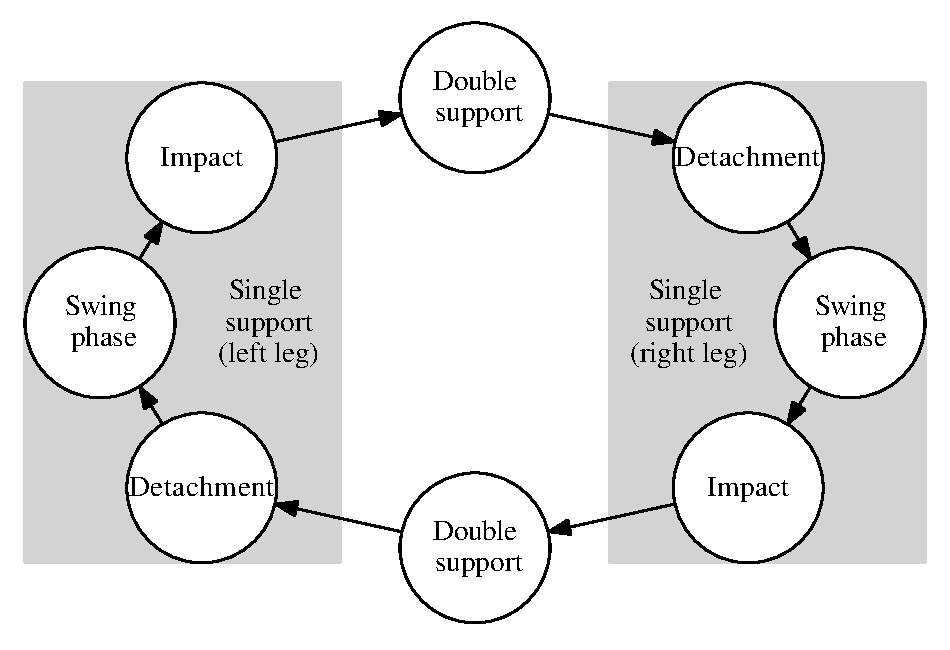
\includegraphics[scale=0.45]{Figures/walk_cycle.eps}}
    \caption[Walking cycle of a biped]{Walking cycle of a biped is typically defined in
    such a way, that it includes two swing phases of right and left leg and two phases 
    when both feet are on the ground.}
    \label{fig.walkcycle}
\end{figure}

The convex hull of the ground contacts in the ground plane is called the {\bf support area}.
In practical applications it is often represented by a polygon, hence an equivalent term 
\ac{PoS} is often used. 

The phase of the walking cycle when only one foot contact with the ground is preserved is
referred to as \ac{SS}, while the phase when both feet are in contact with the ground 
is called \ac{DS}. \ac{SS} and \ac{DS} are also used to denote the respective support area.

{\bf Step} is defined as a half of walking cycle, which includes one single support 
and adjacent double support. {\bf Footstep} denotes the position of a foot in ground plane.
The term ``gait'' is used to denote a pattern of movements of a robot during walk.

In accordance with \cite{VukHumanoidTerms} {\bf balance} is defined as the state, in which 
humanoid preserves the upright position. Some authors use the word ``stability'' instead of 
``balance'', but such use is avoided here to prevent confusion. Terms {\bf static balance} 
and {\bf dynamic balance} are used to discriminate situations when a robot is balanced
while it is still, and while it is moving. The ability to preserve balance is a crucial 
characteristic for walking robots. 


%%%%%%%%%%%%%%%%%%%%%%%%%%%%%%%%%%%%%%%%%%%%%%%%%%%%%%%%%%%%%%%%%%%%%%%%%%%%%%%%
%%%%%%%%%%%%%%%%%%%%%%%%%%%%%%%%%%%%%%%%%%%%%%%%%%%%%%%%%%%%%%%%%%%%%%%%%%%%%%%%
%%%%%%%%%%%%%%%%%%%%%%%%%%%%%%%%%%%%%%%%%%%%%%%%%%%%%%%%%%%%%%%%%%%%%%%%%%%%%%%%
\section{Dynamic Balance}
The dynamic balance of a biped can be ensured using one of the criteria presented
in this section. Note that it is possible to design a gait, which is not balanced
with respect even to the most general criteria mentioned here. For example, a gait
may include a phase of controlled fall, when the fall is started intentionally and 
appropriate preparations are made in order to continue the walk after the foot impact.
Nevertheless, design of such gaits is not a trivial task.

Also, there is a class of robots, which are designed using a completely different
paradigm. Continuous walk of such robots is characterized by a cycle in the phase 
plane, which is supported either naturally or using control \cite{KajitaLegged}. 
{\bf Passive walkers}, which were introduced in \cite{McGeer}, are the best known 
representatives of this class of systems. Walking is a natural dynamic mode of 
passive walkers. Their mechanical design allows them to walk on shallow slopes 
without any active control. Combination of passive dynamics with actuation is also 
a promising research direction \cite{CollinsPassive}. 
% TODO The main disadvantage of the current passive walkers is the lack of agility and responsiveness.


%%%%%%%%%%%%%%%%%%%%%%%%%%%%%%%%%%%%%%%%%%%%%%%%%%%%%%%%%%%%%%%%%%%%%%%%%%%%%%%%
\subsection{Center of Mass}
One of the best known balance criteria is the position of the projection of the \ac{CoM} 
on the ground plane, which must stay within the support area. This criterion was used in 
other engineering disciplines before it was adopted in robotics. Robots that balance 
using projection of \ac{CoM} are called {\bf static walkers} to indicate, that the 
static balance is always preserved. Hence, they can be safely stopped at any moment.

Static walkers are rather limited in their capabilities, in particular their walk is 
rather slow, since they must limit their acceleration. Note that this criterion is 
valid only when all ground contacts of a robot lie on the same horizontal plane 
\cite{WieberStability}.


%%%%%%%%%%%%%%%%%%%%%%%%%%%%%%%%%%%%%%%%%%%%%%%%%%%%%%%%%%%%%%%%%%%%%%%%%%%%%%%%
\subsection{Zero Moment Point}
This criterion, which is based on the existence of \ac{ZMP} \cite{VukZMP35}, was 
proposed by Miomir Vukobratovi\'c in $1968$ at the Third All-Union Congress on 
Theoretical and Applied Mechanics in Moscow. 

The concept of \ac{ZMP} is introduced under the assumption that a robot walks on a flat
floor and the friction forces are strong enough to compensate the ground reaction
forces tangential to the ground.

Since the ground contact of a robot is unilateral (the robot can push on the ground, 
but cannot pull), the only force that can compensate forces that tend to overturn the 
robot is the ground reaction force. The point where the ground reaction force must be 
applied to compensate for other forces must exist within the support area, otherwise 
the robot would lose balance. This point is named \ac{ZMP}.

When the \ac{ZMP} does not exist within the support area, under the assumption that the
support is immobile (which is not true in this case) a \ac{FZMP} can be found in order 
to measure the disbalance \cite{VukHumanoidTerms}.

The position of \ac{CoP}, which is a a point on the ground plane, where the ground 
reaction force is applied, is often considered to be an equivalent of \ac{ZMP}, since they 
coincide while the robot is balanced. Therefore, the actual position of \ac{ZMP} can be 
found using force sensors located on the soles of a robot.

Even though the situation when \ac{ZMP} exists on the edge of the support area do not
necessary lead to fall, it is dangerous since any small disturbance may overturn
the robot. The easiest way to avoid this is to define support area with a safety 
margin.


%%%%%%%%%%%%%%%%%%%%%%%%%%%%%%%%%%%%%%%%%%%%%%%%%%%%%%%%%%%%%%%%%%%%%%%%%%%%%%%%
\subsection{Other Criteria}
The forenamed criteria cannot be used on uneven terrain, but a more general criteria
can be developed \cite{WieberStability, BretlEquilibrium, AdiosZMP}. Nevertheless,
they are computationally more expensive and may be infeasible for real-time applications
\cite{WieberStability}. 

%Some authors have also extended \ac{ZMP} heuristically \cite{SardainZMP}.



%%%%%%%%%%%%%%%%%%%%%%%%%%%%%%%%%%%%%%%%%%%%%%%%%%%%%%%%%%%%%%%%%%%%%%%%%%%%%%%%
%%%%%%%%%%%%%%%%%%%%%%%%%%%%%%%%%%%%%%%%%%%%%%%%%%%%%%%%%%%%%%%%%%%%%%%%%%%%%%%%
%%%%%%%%%%%%%%%%%%%%%%%%%%%%%%%%%%%%%%%%%%%%%%%%%%%%%%%%%%%%%%%%%%%%%%%%%%%%%%%%
\section{3D Linear Inverted Pendulum Model}\label{sec.3dlipm}
Apart from balancing there are other factors that complicate control of walking
robots. Hence, it is common to make simplifying assumptions. For example, in this
thesis it is assumed that walk is performed in such a way, that constraints 
imposed by environment, joint limits, self-collision avoidance are never violated.

However, it is necessary to make other assumptions. Consider generation of trajectories
for a humanoid in the joint or operational space. If these trajectories are generated
offline, the motion cannot adapt to the walk conditions. Hence, it is more appealing to 
generate motion profiles online. This can be achieved with the help of \ac{MPC} 
\cite{KajitaLegged}, refer to \cref{ch.MPC} for more information on \ac{MPC}. If the whole 
model of a robot robot is incorporated in the \ac{MPC}, then the respective optimization 
problem becomes nonlinear \cite{KajitaLegged}. Real-time control based on \ac{NMPC} is 
not always feasible, since its application is a computationally expensive task. This 
limitation motivated researchers to develop control schemes that avoid \ac{NMPC} and 
use simple \ac{LMPC} instead.

The dynamics of a humanoid walking on a flat ground can be approximated (in a reasonable 
way) by a linear model, which is called \ac{3D-LIPM} \cite{3d-lipm}. This model is based 
on two important assumptions. The first one allows to ignore the structure of the robot 
in order to represent it by an inverted pendulum. The second one restricts motions of 
pendulum to a plane in order to obtain linear model. Though, this plane can be inclined, 
henceforth it is assumed to be parallel to the ground surface and intersect the $z$ axis
at the height of \ac{CoM} $c^z$.

The \ac{3D-LIPM} system must be controlled using torques. For convenience, the torques
can be expressed through the coordinates of \ac{ZMP} leading to {\bf cart-on-a-table 
model} \cite{LIPM-MPC}. This model allows computation of \ac{ZMP} position using
\begin{equation}\label{eq.zmp_cart}
\begin{split}
z^x &= c^x - h \ddot{c}^x, \\
z^y &= c^y - h \ddot{c}^y, \\
\end{split}
\end{equation}
where 
$$
h = \frac{c^z}{g};
$$
$(z^x, z^y)$ and $(c^x, c^y)$ are coordinates of \ac{ZMP} and \ac{CoM} on the 
horizontal plane; $(\ddot{c}^x, \ddot{c}^y)$ are the accelerations of \ac{CoM} 
on the horizontal plane; $g = 9.8$ is gravitational acceleration; $c^z$ is the height
of the plane, in which motion of the \ac{CoM} is constrained.

Based on the \cref{eq.zmp_cart} a discrete-time time-invariant linear dynamical 
system can be obtained using trivial integration
\begin{equation}\label{eq.system_orig}
\begin{split}
\hat{\mbm{c}}_{k+1} &= \mbm{A}\hat{\mbm{c}}_{k}+\mbm{B}\dddot{\mbm{c}}_{k}\\
\mbm{z}_k &= \mbm{C} \hat{\mbm{c}}_{k}.
\end{split}
\end{equation}
Where the state
$$
\hat{\mbm{c}}_{k} = 
\begin{bmatrix} 
c_k^x & \dot{c}_k^x & \ddot{c}_k^x & c_k^y & \dot{c}_k^y & \ddot{c}_k^y
\end{bmatrix}^T
$$
includes the position, velocity, and acceleration of \ac{CoM}; and the control
vector
$$
\dddot{\mbm{c}}_{k} = \begin{bmatrix} \dddot{c}_k^x & \dddot{c}_k^y \end{bmatrix}^T;
$$
consists of jerks of \ac{CoM}.
State transition and control input matrices are
$$
\mbm{A} = 
\begin{bmatrix}
    1 & T & T^{2}/2 & 0 & 0 & 0\\ 
    0 & 1 & T & 0 & 0 & 0\\ 
    0 & 0 & 1 & 0 & 0 & 0\\
    0 & 0 & 0 & 1 & T & T^{2}/2\\
    0 & 0 & 0 & 0 & 1 & T\\
    0 & 0 & 0 & 0 & 0 & 1
\end{bmatrix}, \quad
\mbm{B} =
\begin{bmatrix}
    T^{3}/6 & 0\\ 
    T^{2}/2 & 0\\
    T      & 0\\
    0      & T^{3}/6\\
    0      & T^{2}/2\\
    0      & T
\end{bmatrix},
$$
where $T$ is the length of a discretization step in seconds; and the output matrix is
$$
\mbm{C} = 
\begin{bmatrix}
    1 & 0 & -h & 0 & 0 & 0\\ 
    0 & 0 & 0  & 1 & 0 & -h\\
\end{bmatrix}.
$$
The system~\eqref{eq.system_orig} is suitable for implementation of an \ac{MPC} 
controller for \ac{CoM} and \ac{ZMP} trajectory generation. 

Another approach to generation of these trajectories is based on analytical 
solutions of the differential equations~\eqref{eq.zmp_cart}, for example refer to 
\cite{MorisawaAnalytical,LiuAnalytical}. In this case the \ac{ZMP} trajectory 
can be represented by a polynomial. 
%This approach can be preferrable in situations,
%when the future footsteps are not known. When \ac{MPC} scheme is used, at least
%several footsteps must be defined in advance (the reason is explained in 
%\cref{sec.mpc_stability}).


%%%%%%%%%%%%%%%%%%%%%%%%%%%%%%%%%%%%%%%%%%%%%%%%%%%%%%%%%%%%%%%%%%%%%%%%%%%%%%%%
%%%%%%%%%%%%%%%%%%%%%%%%%%%%%%%%%%%%%%%%%%%%%%%%%%%%%%%%%%%%%%%%%%%%%%%%%%%%%%%%
%%%%%%%%%%%%%%%%%%%%%%%%%%%%%%%%%%%%%%%%%%%%%%%%%%%%%%%%%%%%%%%%%%%%%%%%%%%%%%%%
\section{Nao Overview}\label{sec.nao}
The experimental part of this thesis was conducted on a Nao robot. A software 
module developed for control of this robot is described in \cref{ch.naomodule}.

\begin{figure}[ht]
    \centerline{%
    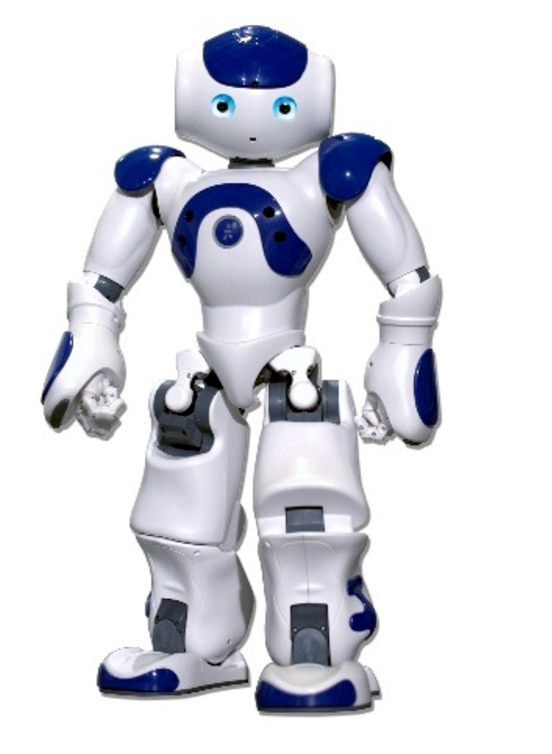
\includegraphics[scale=0.35]{Figures/nao.eps}}
    \caption[The Nao robot]{The Nao robot. The walking pattern generator that was 
    developed during the work on the thesis was tested on a Nao robot.}
    \label{fig.nao}
\end{figure}
Nao (see \cref{fig.nao}) is a small, fully actuated, position-controlled humanoid 
robot developed by a french company Aldebaran Robotics. We are working with 
version $3.2$ of this robot, which is $58$ centimeters tall, weights about $4.5$ 
kilograms and has $25$ degrees of freedom. The parameters of the processor installed
on this version of Nao is given in \cref{tbl.cpu}.

\begin{table}
\begin{center}
\begin{tabular}{c|p{7cm}}
model name & Geode(TM) Integrated Processor by AMD PCS\\
cpu MHz    & 499.903\\
cache size & 128 KB\\
flags      & fpu de pse tsc msr cx8 sep pge cmov clflush
             mmx mmxext 3dnowext 3dnow\\
\end{tabular}
\caption[The Nao CPU information]{The Nao CPU information.}
\label{tbl.cpu}
\end{center}
\end{table}

The operating system of the Nao robots is based on Linux. Various functionalities 
of Nao are provided by modules, which run within \verb|NaoQI| framework on Nao or 
a computer. Modules communicate with each other transparently through special 
application programming interface. \verb|NaoQI| framework supports modules written 
in \verb|C++| or \verb|python|. In order to build modules that must run on the
robot, the \ac{SDK} is required. The fresh releases of the operating system, the 
\ac{SDK}, and a comprehensive documentation\footnote{The Nao software documentation 
is available on the website of Aldebaran Robotics at
\url{http://www.aldebaran-robotics.com/documentation/index.html}.}
can be obtained from Aldebaran Robotics. The version of \ac{SDK} and operating system, 
which were used for development and tests, is $1.12$.

The standard software distribution for the Nao robots includes a walking module,
which uses the control scheme described in \cite{NaoWalk}.

%-------------------------------------------------------------------------------
\chapter{Formulation of Model Predictive Control Problem}
\label{ch.MPC}
%-------------------------------------------------------------------------------
Model predictive control \cite{MacMPC} is a mature and widely used control 
paradigm. Its name points to two important characteristics: this strategy
is based on the knowledge of the model of the underlying process, and the behavior
of the system is predicted over some preview horizon. The goal of \ac{MPC} is to
choose a sequence of control inputs for the system over prediction horizon with
respect to given objective function and constraints. This goal can be informally
interpreted as choosing such control inputs, that do not lead to undesirable 
effects in the future. The problem is resolved periodically in order to 
accommodate for the current situation, the preview window is usually shifted in 
time on each iteration of \ac{MPC}. 

Generation of \ac{CoM} and \ac{ZMP} trajectories using an \ac{MPC} scheme was
proposed in \cite{LIPM-MPC}. This chapter reviews some extensions of the scheme
introduced in \cite{WieberMPC, dimitrov2011sparse}.



%%%%%%%%%%%%%%%%%%%%%%%%%%%%%%%%%%%%%%%%%%%%%%%%%%%%%%%%%%%%%%%%%%%%%%%%%%%%%%%%
%%%%%%%%%%%%%%%%%%%%%%%%%%%%%%%%%%%%%%%%%%%%%%%%%%%%%%%%%%%%%%%%%%%%%%%%%%%%%%%%
%%%%%%%%%%%%%%%%%%%%%%%%%%%%%%%%%%%%%%%%%%%%%%%%%%%%%%%%%%%%%%%%%%%%%%%%%%%%%%%%
\section{Unconstrained Model Predictive Control Formulation}
The original \ac{MPC} problem defined in \cite{LIPM-MPC} has finite horizon, a 
quadratic objective function, and is based on a discrete system~\eqref{eq.system_orig}. 
The objective function penalizes distance from predefined reference points for \ac{ZMP}, 
the change in state and control. Since this formulation has no inequality constraints 
an explicit control law ({\bf linear quadratic regulator}) was obtained.

Consider the unconstrained \ac{MPC} based on the system~\eqref{eq.system_orig}
where the objective function is defined equivalently to the objective function
used in \cite{WieberMPC}.
\begin{equation}\label{eq.opt_simple}
\begin{split}
\minimize{\dddot{\mbm{c}}_0 \dots \dddot{\mbm{c}}_{N-1}; \hat{\mbm{c}}_1 \dots \hat{\mbm{c}}_{N}}
            & \frac{1}{2} \sum_{k=1}^{N}   \norm{ \mbm{C} \hat{\mbm{c}}_{k} - \mbm{z}_k^{ref} }^2_{\mbm{Q}} 
            + \frac{1}{2} \sum_{k=0}^{N-1} \norm{ \dddot{\mbm{c}}_k }^2_{\mbm{P}}\\
\subjectto  & \hat{\mbm{c}}_{k+1} = \mbm{A}\hat{\mbm{c}}_{k}+\mbm{B}\dddot{\mbm{c}}_{k},\\
\end{split}
\end{equation}
where 
$$
\mbm{C} = 
\begin{bmatrix}
    1 & 0 & -h & 0 & 0 & 0\\ 
    0 & 0 & 0  & 1 & 0 & -h\\
\end{bmatrix}.
$$
$N$ is the number of sampling intervals in the preview window, matrices $\mbm{Q}$ 
and $\mbm{P}$ contain gains, $\mbm{z}_k^{ref}$ are reference positions for \ac{ZMP}
at discrete sampling time $k$. The objective function does not penalize the change 
in the state $\hat{\mbm{c}}_{k}$, and penalizes the absolute values of control 
inputs instead of change between subsequent control inputs.


%%%%%%%%%%%%%%%%%%%%%%%%%%%%%%%%%%%%%%%%%%%%%%%%%%%%%%%%%%%%%%%%%%%%%%%%%%%%%%%%
%%%%%%%%%%%%%%%%%%%%%%%%%%%%%%%%%%%%%%%%%%%%%%%%%%%%%%%%%%%%%%%%%%%%%%%%%%%%%%%%
%%%%%%%%%%%%%%%%%%%%%%%%%%%%%%%%%%%%%%%%%%%%%%%%%%%%%%%%%%%%%%%%%%%%%%%%%%%%%%%%
\section{Introducing the Inequality Constraints}\label{sec.ds_constraints}
The authors of \cite{WieberMPC} impose constraints on the position of \ac{ZMP}
in order to keep it within the support area and demonstrate that a robot can cope 
with stronger disturbances in this case. Computation of explicit control law for 
\ac{MPC} with inequality constraints \cite{BemporadConstrLQR} is not possible here, 
since the constraints change on each iteration.

Therefore, the application of MPC requires the solution of a quadratic programming 
problem. The quadratic programming is discussed in \cref{ch.QP}. This section is 
focused on the formulation of \ac{MPC} for \ac{CoM}/\ac{ZMP} trajectory generation 
with inequality constraints on \ac{ZMP} positions. This \ac{MPC} is referred to in 
the thesis as \ac{MPCWMG}.


%%%%%%%%%%%%%%%%%%%%%%%%%%%%%%%%%%%%%%%%%%%%%%%%%%%%%%%%%%%%%%%%%%%%%%%%%%%%%%%%
\subsection{Double Support Constraints}
Note that the support area differs depending on the type of support. \ac{SS} can 
be easily represented by a rectangle, while \ac{DS} in a general case cannot. 
Therefore, we need to find a suitable representation of \ac{DS} constraints.

The support area in \ac{DS} is the convex hull of two adjacent \ac{SS}. When the 
\ac{SS} constraints are rectangular, their convex hull is a polygon as shown in 
\cref{fig.ds_hull}. In this case the constraints for \ac{SS} and \ac{DS} must 
be handled differently. We introduce an approximation of this convex hull by
a sequence of rectangles, as demonstrated in \cref{fig.ds_approx}. This approach
allows to define constraints uniformly, furthermore, it makes possible an 
extension of the \ac{MPCWMG} to perform footstep repositioning to compensate for
disturbances \cite{dimitrov2011walking}.
\begin{figure}[ht]
\begin{minipage}[b]{0.4\linewidth}
    \centerline{%
    \includegraphics[scale=0.4]{Figures/ds_convex_hull.eps}}
    \caption[Double support]{A double support represented by a convex hull of two single supports}
    \label{fig.ds_hull}
\end{minipage}
\hfill
\begin{minipage}[b]{0.4\linewidth}
    \centerline{%
    \includegraphics[scale=0.4]{Figures/ds_approx.eps}}
    \caption[Approximate double support]{A double support approximated by a sequence of rectangles}
    \label{fig.ds_approx}
\end{minipage}
\end{figure}


%%%%%%%%%%%%%%%%%%%%%%%%%%%%%%%%%%%%%%%%%%%%%%%%%%%%%%%%%%%%%%%%%%%%%%%%%%%%%%%%
\subsection{Definition of the Inequality Constraints}
A rectangle can be defined with respect to some reference frame $\mathbb{F}$ by
four positive distances 
$\mbm{d} = \begin{bmatrix} u^x & u^y & -l^x & -l^y \end{bmatrix}^T$ 
from the origin of $\mathbb{F}$ to the edges of the rectangle. The position and
orientation of the rectangle are given by the displacement $\mbm{r}$ and angle 
of rotation $\varphi$ of $\mathbb{F}$ with respect to the global reference frame. 
An example is depicted in \cref{fig.constr}.

\begin{figure}[ht]
    \psfragscanon
    \psfrag{r}{$\mbm{r}$}
    \psfrag{a}{$\varphi$}
    \psfrag{h}{$u^x$}
    \psfrag{j}{$u^y$}
    \psfrag{k}{$-l^x$}
    \psfrag{l}{$-l^y$}
    \centerline{%
    \includegraphics[scale=0.5]{Figures/rect_constraints.eps}}
    \caption[Support rectangle]{Definition of a support rectangle with respect to the global reference frame}
    \label{fig.constr}
\end{figure}

All points $\mbm{p}$ lying within the rectangle satisfy
$$
\mbm{D}\mbm{R}^T\left(\mbm{p} - \mbm{r} \right) \leq \mbm{d},
$$
where matrix $\mbm{D}$ and rotation matrix $\mbm{R}$ are defined as
$$
\mbm{D} = 
\begin{bmatrix}
    \mbm{I}\\
    -\mbm{I}
\end{bmatrix}, \quad
%
\mbm{R} =
\begin{bmatrix}
    \cos\varphi & -\sin\varphi \\
    \sin\varphi & \cos\varphi
\end{bmatrix}.
$$

Thus the constraints for the $k$-th sampling period in the preview window are
\begin{equation}
\mbm{D}\mbm{R}^T_k \mbm{C} \hat{\mbm{c}}_k \leq \mbm{d}_{k} + \mbm{D}\mbm{R}^T_k \mbm{r}_k,
\end{equation}
where 
$$
\mbm{C} = 
\begin{bmatrix}
    1 & 0 & -h & 0 & 0 & 0\\ 
    0 & 0 & 0  & 1 & 0 & -h\\
\end{bmatrix}.
$$
is the output matrix of the system~\ref{eq.system_orig} defined in \cref{sec.3dlipm}.


%%%%%%%%%%%%%%%%%%%%%%%%%%%%%%%%%%%%%%%%%%%%%%%%%%%%%%%%%%%%%%%%%%%%%%%%%%%%%%%%
%%%%%%%%%%%%%%%%%%%%%%%%%%%%%%%%%%%%%%%%%%%%%%%%%%%%%%%%%%%%%%%%%%%%%%%%%%%%%%%%
%%%%%%%%%%%%%%%%%%%%%%%%%%%%%%%%%%%%%%%%%%%%%%%%%%%%%%%%%%%%%%%%%%%%%%%%%%%%%%%%
\section{Time-variant Constrained MPC}\label{sec.timevarsys}
We can exclude the dynamics of the system~\eqref{eq.system_orig} from the inequality 
constraints by replacing the position of the \ac{CoM} by the position of the \ac{ZMP} 
so that
\begin{equation}\label{eq.substitution1}
\tilde{\mbm{c}} = 
\begin{bmatrix} z^x & \dot{c}^x & \ddot{c}^x & z^y & \dot{c}^y & \ddot{c}^y \end{bmatrix}^T,
\end{equation}
to obtain
\begin{equation}\label{eq.constraints}
\mbm{D}\mbm{R}^T_k \mbm{C}_p \tilde{\mbm{c}}_k \leq \mbm{d}_{k} + \mbm{D}\mbm{R}^T_k \mbm{r}_k,
\end{equation}
where
$$
\mbm{C}_p =
\begin{bmatrix}
    1 & 0 & 0 & 0 & 0 & 0 \\
    0 & 0 & 0 & 1 & 0 & 0 \\
\end{bmatrix},
$$

The system must be changed accordingly
\begin{equation}\label{eq.system_sub1}
\tilde{\mbm{c}}_{k+1} = \tilde{\mbm{A}}_k\tilde{\mbm{c}}_{k} + \tilde{\mbm{B}}_k\dddot{\mbm{c}}_{k},
\end{equation}
where the state transition and control matrices are defined as 
$$
\tilde{\mbm{A}}_k =
\begin{bmatrix}
    1 & T_k & \frac{T_k^{2}}{2}-\Delta h_k & 0 & 0 & 0\\ 
    0 & 1 & T_k & 0 & 0 & 0\\ 
    0 & 0 & 1 & 0 & 0 & 0\\
    0 & 0 & 0 & 1 & T_k & \frac{T_k^{2}}{2}-\Delta h_k\\
    0 & 0 & 0 & 0 & 1 & T_k\\
    0 & 0 & 0 & 0 & 0 & 1
\end{bmatrix},
$$
$$
\tilde{\mbm{B}}_k = 
\begin{bmatrix}
    \frac{T_k^{3}}{6} - h_k T_k     & 0\\ 
    \frac{T_k^{2}}{2}               & 0\\ 
    T_k                             & 0\\
    0                               & \frac{T_k^{3}}{6} - h_k T_k\\
    0                               & \frac{T_k^{2}}{2}\\
    0                               & T_k
\end{bmatrix}.
$$
These matrices can be defined as time-invariant, but their parameterization gives us more options 
for tuning. Variation of the \ac{CoM} height during walk, which can be realized through the
appropriate changes of $h_k$, may have a positive effect on the quality of the gait. Also,
the solution of the \ac{QP} may be obtained faster, if the sampling time $T_k$ varies in 
the preview window. Note that the duration of the sampling period in an \ac{MPC} is determined 
by the control sampling time, and all but the first computed control inputs are usually 
discarded. Hence, longer sampling periods in the end of the preview window can be used to 
decrease $N$, which directly affects the time required for solution, without decreasing the 
length of this preview window \cite{dimitrov2008implementation}.

Now we rewrite the optimization problem~\eqref{eq.opt_simple} to reflect the changes 
in the model
\begin{equation}\label{eq.opt}
\begin{split}
\minimize{\dddot{\mbm{c}}_0 \dots \dddot{\mbm{c}}_{N-1}; \tilde{\mbm{c}}_1 \dots \tilde{\mbm{c}}_{N}}
            & \sum_{k=1}^{N}    \norm{ \tilde{\mbm{c}}_k - \mbm{C}_p^T \mbm{z}_k^{ref} }^2_{\tilde{\mbm{Q}}} 
            + \sum_{k=0}^{N-1}  \norm{ \dddot{\mbm{c}}_k }^2_{\mbm{P}}\\ 
\subjectto  & \tilde{\mbm{c}}_{k+1} = \tilde{\mbm{A}}_k\tilde{\mbm{c}}_{k} + \tilde{\mbm{B}}_k\dddot{\mbm{c}}_{k}\\
            & \mbm{D}\mbm{R}^T_k \mbm{C}_p \tilde{\mbm{c}}_k \leq \mbm{d}_{k} + \mbm{D}\mbm{R}^T_k \mbm{r}_k, 
\end{split}
\end{equation}
where the gain matrices are
$$
\tilde{\mbm{Q}} =
\begin{bmatrix}
    \frac{\alpha_g}{2} & 0                 & 0 & 0 & 0 & 0\\ 
    0               & \frac{\beta_g}{2}  & 0 & 0 & 0 & 0\\ 
    0               & 0                 & \frac{\gamma_g}{2} & 0 & 0 & 0\\ 
    0 & 0 & 0 & \frac{\alpha_g}{2} & 0                 & 0 \\ 
    0 & 0 & 0 & 0               & \frac{\beta_g}{2}  & 0 \\ 
    0 & 0 & 0 & 0               & 0                 & \frac{\gamma_g}{2} \\ 
\end{bmatrix}, \quad
\mbm{P} = 
\begin{bmatrix}
      \frac{\eta_g}{2}  & 0  \\ 
      0                 &  \frac{\eta_g}{2} \\ 
\end{bmatrix}.
$$

The first term in the objective function is
\begin{equation*}
\begin{split}
    \sum_{k=1}^{N} \norm{ \tilde{\mbm{c}}_k - \mbm{C}_p^T \mbm{z}_k^{ref} }^2_{\tilde{\mbm{Q}}} &=
    \sum_{k=1}^{N} \left(
        \norm{ \tilde{\mbm{c}}_k }^2_{\tilde{\mbm{Q}}} 
        + \norm{ \mbm{C}_p^T \mbm{z}_k^{ref} }^2_{\tilde{\mbm{Q}}}
        - 2 \tilde{\mbm{c}}_k^T \tilde{\mbm{Q}} \mbm{C}_p^T \mbm{z}_k^{ref}
    \right)\\
    &= \sum_{k=1}^{N} \left(
        \norm{ \tilde{\mbm{c}}_k }^2_{\tilde{\mbm{Q}}} 
        + \norm{ \mbm{C}_p^T \mbm{z}_k^{ref} }^2_{\tilde{\mbm{Q}}}
        - \alpha_g (\mbm{C}_p^T \mbm{z}_k^{ref})^T \tilde{\mbm{c}}_k
    \right)\\
    &= \sum_{k=1}^{N} \left(
        \norm{ \tilde{\mbm{c}}_k }^2_{\tilde{\mbm{Q}}} 
        + \norm{ \mbm{C}_p^T \mbm{z}_k^{ref} }^2_{\tilde{\mbm{Q}}}
        + \mbm{q}_k^T \tilde{\mbm{c}}_k
    \right),
\end{split}
\end{equation*}
where $\mbm{q}_k = - \alpha_g (\mbm{C}_p^T \mbm{z}_k^{ref})$.

The terms $\norm{ \mbm{C}_p^T \mbm{z}_k^{ref} }^2_{\tilde{\mbm{Q}}}$ are constant
and can be dropped. Thus we obtain the following formulation \ac{MPCWMG}
\begin{equation}\label{eq.opt_final}
\begin{split}
\minimize{\dddot{\mbm{c}}_0 \dots \dddot{\mbm{c}}_{N-1}; \tilde{\mbm{c}}_1 \dots \tilde{\mbm{c}}_{N}}
            & \sum_{k=1}^{N}    \norm{ \tilde{\mbm{c}}_k }^2_{\tilde{\mbm{Q}}} 
            + \sum_{k=0}^{N-1}  \norm{ \dddot{\mbm{c}}_k }^2_{\mbm{P}} 
            + \sum_{k=1}^{N}    \mbm{q}_k^T \tilde{\mbm{c}}_k\\
\subjectto  & \tilde{\mbm{c}}_{k+1} = \tilde{\mbm{A}}_k\tilde{\mbm{c}}_{k} + \tilde{\mbm{B}}_k\dddot{\mbm{c}}_{k}\\
            & \mbm{D}\mbm{R}^T_k \mbm{C}_p \tilde{\mbm{c}}_k \leq \mbm{d}_{k} + \mbm{D}\mbm{R}^T_k \mbm{r}_k.
\end{split}
\end{equation}


%%%%%%%%%%%%%%%%%%%%%%%%%%%%%%%%%%%%%%%%%%%%%%%%%%%%%%%%%%%%%%%%%%%%%%%%%%%%%%%%
%%%%%%%%%%%%%%%%%%%%%%%%%%%%%%%%%%%%%%%%%%%%%%%%%%%%%%%%%%%%%%%%%%%%%%%%%%%%%%%%
%%%%%%%%%%%%%%%%%%%%%%%%%%%%%%%%%%%%%%%%%%%%%%%%%%%%%%%%%%%%%%%%%%%%%%%%%%%%%%%%
\section{Generation of an Initial Guess}\label{sec.init_guess}
The \ac{MPC} problem~\eqref{eq.opt_final} is always feasible. This is a useful
property for generation of an initial feasible point.

At each iteration of \ac{MPCWMG} the current state of the system~\eqref{eq.system_sub1}
is assumed to be known. It is also possible to find a set of $N$ points satisfying the
inequality constraints~\eqref{eq.constraints} for each sampling period. This
set is a feasible profile for \ac{ZMP}, the next step is to generate control inputs 
to follow this profile and determine the unknown state variables using a simple
iterative procedure.

The $k$-th control inputs can be computed based on the current state and the next 
\ac{ZMP} position by multiplying both sides of \cref{eq.system_sub1} by $\mbm{C}_p$
$$
\dddot{\mbm{c}}_{k} = (\mbm{C}_p\tilde{\mbm{B}}_k)^{-1} (\mbm{z}_{k+1} 
                    - \mbm{C}_p \tilde{\mbm{A}}_k\tilde{\mbm{c}}_{k}).
$$
Matrix $\mbm{C}_p\tilde{\mbm{B}}_k$ is not invertible when $c^z_k = T_k^2 / 6$.
If the sampling period is less than $0.1$ second, then the height of \ac{CoM} 
of a robot must be lower than approximately $2$ millimeters in order to satisfy 
this equality. Since the sampling period used in simulations and experiments is 
always below $0.1$ second, it is safe to assume that the matrix is always invertible.

Having the $k$-th control inputs and the current state it is possible to find 
velocity and acceleration of the next state using \cref{eq.system_sub1}.


%%%%%%%%%%%%%%%%%%%%%%%%%%%%%%%%%%%%%%%%%%%%%%%%%%%%%%%%%%%%%%%%%%%%%%%%%%%%%%%%
%%%%%%%%%%%%%%%%%%%%%%%%%%%%%%%%%%%%%%%%%%%%%%%%%%%%%%%%%%%%%%%%%%%%%%%%%%%%%%%%
%%%%%%%%%%%%%%%%%%%%%%%%%%%%%%%%%%%%%%%%%%%%%%%%%%%%%%%%%%%%%%%%%%%%%%%%%%%%%%%%
\section{Stability of the MPC scheme}\label{sec.mpc_stability}
When an \ac{MPC} with finite horizon is used, its stability must be considered.
It is possible to ensure stability using appropriate modifications of the problem,
for a comprehensive review refer to \cite{MPCstab}. Stability of the \ac{MPC} 
formulations presented so far is not guaranteed. Moreover, it is difficult to
judge on the stability of the \ac{MPCWMG}, since the problem is altered on each 
iteration due to the change of the set of the inequality constraints.

Let us neglect the changes of the constraints for the moment and consider the 
\ac{QP} problem, which is solved on a particular iteration. Note that the discrete 
systems~\eqref{eq.system_orig} and~\eqref{eq.system_sub1} are unstable, since the 
state transition matrices have repeated eigenvalues equal to $1$ and the dimesion 
of the respective Jordan blocks is greater than $1$. Consequently, it is necessary to 
impose terminal constraints in order to ensure stability \cite{MuskeLinearMPC}. 
\ac{QP} with terminal constraints may become infeasible, and generation of an initial 
guess (\cref{sec.init_guess}) may become more computationally expensive. The stable 
\ac{MPCWMG} may improve the ability of a robot to cope with external disturbances 
and may require shorter preview window. However, the effect on the quality of the 
gait is unknown. Furthermore, the stability of \ac{MPCWMG} does not imply, that the 
generated \ac{CoM} trajectory can be executed by the controlled robot. Hence, the 
stability of the \ac{MPCWMG} scheme requires special consideration and experiments, 
and it was decided to leave it out of the scope of the thesis.

In order to avoid stability issues a ``sufficiently long'' preview window is
used. In \cite{LIPM-MPC}, where \ac{MPC} problem is not constrained, the explicit 
control law was computed, and the preview gain was shown to be decreasing to a very
small value in about $2$ seconds. The built-in walking module for Nao uses preview 
window of $0.8$ second \cite{NaoWalk}. In a similar way, the necessary preview window 
length for the developed walking module was found experimentally (it is about $1.6$ 
second, see \cref{ch.results}). Since this time is related to the speed of walk, 
the number of footsteps is likely to be a better measure of a preview horizon. In our 
implementation $1.6$ second includes three \ac{SS}, or one full oscillation of the 
\ac{ZMP} trajectory.

% {\bf robust} \ac{MPC} and {\bf stochastic} \ac{MPC}
%orbital stability
%constraints on z vs c cddot
%\cite{RaoIPMPC}

%-------------------------------------------------------------------------------
\chapter{Solving the Quadratic Problem}
\label{ch.QP}
%-------------------------------------------------------------------------------
%TODO backtracking search
In \cref{ch.MPC} it was pointed out that \ac{MPCWMG} requires solution of a \ac{QP}
on each iteration. The theory and algorithms for this class of optimization problems
are well developed \cite{NocedalNumOpt, BoydCVX}. 

We implemented {\bf primal active set} and {\bf primal interior point} methods for 
the solution of \ac{QP}. Comparison of these two methods with respect to solution 
of \ac{MPCWMG} is given in \cref{ch.results}. One of these methods can be preferable
depending on the \ac{QP}. One iteration of the interior point method is more expensive, 
but it has polynomial complexity, while the active set method has exponential complexity 
\cite{RaoIPMPC}. Consequently, the active set method can be faster for the problems
with relatively small number of inequality constraints \cite{BartlettASvsIP}. The 
primal methods are preferred to the dual methods, since each iteration of the former 
produce a sub-optimal solution that can be used instead of the solution. Note that 
primal strategies require feasible initial point, which can be easily generated for 
\ac{MPCWMG} as described in \cref{sec.init_guess}.

The formulations that are used for implementation of active set and logarithmic
barrier methods presented in this chapter have certain differences. These 
differences do not alter the quadratic problem~\eqref{eq.opt_final}, but make 
implementation more convenient or improve performance.



%%%%%%%%%%%%%%%%%%%%%%%%%%%%%%%%%%%%%%%%%%%%%%%%%%%%%%%%%%%%%%%%%%%%%%%%%%%%%%%%
%%%%%%%%%%%%%%%%%%%%%%%%%%%%%%%%%%%%%%%%%%%%%%%%%%%%%%%%%%%%%%%%%%%%%%%%%%%%%%%%
%%%%%%%%%%%%%%%%%%%%%%%%%%%%%%%%%%%%%%%%%%%%%%%%%%%%%%%%%%%%%%%%%%%%%%%%%%%%%%%%
\section{Fast Solution of MPC Problems}
It was demonstrated in \cite{Nishiwaki}, that a short sampling period is desirable
for control of a walking robot. However, strict time constraints are imposed on
the solution of \ac{MPCWMG} in this case. Hence it is necessary to utilize some
of the techniques that were developed in order to improve performance of the 
\ac{MPC} solvers with short sampling periods. In this section only the general 
techniques are discussed, while more specific optimizations and tuning are described 
later in this chapter and \cref{ch.results}.

The \ac{MPC} problems are often reformulated in order to reduce the number of 
decision variables, since it is possible to express the state variables through 
the control inputs and eliminate the equality constraints. This process is sometimes
referred to as {\bf condensing} \cite{FerreauASWarm, BockMultShooting}. Though the 
number of decision variables is smaller in this case, the problem (its Hessian and 
constraints) is less structured. Furthermore, in many cases condensing is performed
offline, since it is computationally expensive. This imposes unnecessary limitations,
for example, the Hessian is computed for the fixed height of \ac{CoM}. Alternatively, 
it is possible to solve the problem in the same form as given in \cref{eq.opt_final} 
and exploit the structure of the problem. A solver, which is aware of the structure 
of the problem, can be faster, since the number of floating point operations per one 
sampling interval is reduced \cite{FastMPC, dimitrov2011sparse, RaoIPMPC}. The 
approach, which eliminates the equality constraints, in general yields a dense 
Hessian matrix, while the other one preserves block-diagonal structure of the 
Hessian. We discriminate these two approaches by calling them {\bf dense} and 
{\bf sparse}, respectively. Some authors use terms {\bf sequential} and 
{\bf simultaneous} for this purpose \cite{DiehlNMPC}. In \cite{dimitrov2011sparse} 
we showed how sparse formulation can be applied to \ac{MPCWMG}.

{\bf Warm-start} techniques can also leverage the performance of the \ac{MPC} solvers.
These techniques accelerate the computation of the solution on iteration $k+1$ using 
the data obtained on the $k$-th iteration. Warm-start techniques are not adopted in
the implementation of the solvers.

In some cases it is impossible to find the solution of \ac{QP} in the available
time, but a sub-optimal solution is admissible. Such sub-optimal solution can be
obtained, when a primal quadratic programming method (either active set or logarithmic
barrier method) is interrupted at some intermediate iteration. This strategy was used 
in the experiments described in \cref{ch.results}.



%%%%%%%%%%%%%%%%%%%%%%%%%%%%%%%%%%%%%%%%%%%%%%%%%%%%%%%%%%%%%%%%%%%%%%%%%%%%%%%%
%%%%%%%%%%%%%%%%%%%%%%%%%%%%%%%%%%%%%%%%%%%%%%%%%%%%%%%%%%%%%%%%%%%%%%%%%%%%%%%%
%%%%%%%%%%%%%%%%%%%%%%%%%%%%%%%%%%%%%%%%%%%%%%%%%%%%%%%%%%%%%%%%%%%%%%%%%%%%%%%%
\section{Quadratic Problem in a Matrix Form}
In the derivations presented in this chapter it is more convenient to work with 
the \ac{MPCWMG}~\eqref{eq.opt_final}, when \ac{QP} is written in a matrix form. 

Let us define the state vector as
$$
\mbm{x} = \begin{bmatrix} \tilde{\mbm{v}}_c \\ \mbm{v}_u \end{bmatrix},
$$
where
$$
\quad
\tilde{\mbm{v}}_c = \begin{bmatrix} \tilde{\mbm{c}}_1 \\ \vdots \\ \tilde{\mbm{c}}_N \end{bmatrix} , \quad
\mbm{v}_u = \begin{bmatrix} \dddot{\mbm{c}}_1 \\ \vdots \\ \dddot{\mbm{c}}_N \end{bmatrix} .
$$

The objective function in a matrix form is
$$
f\left(\tilde{\mbm{v}}_c, \mbm{v}_u\right) =
\begin{bmatrix} \tilde{\mbm{v}}_c \\ \mbm{v}_u \end{bmatrix}^T
\begin{bmatrix} 
    \tilde{\mbm{H}}_c   & \mbm{0} \\ 
    \mbm{0}             & \mbm{H}_u \\
\end{bmatrix}
\begin{bmatrix} \tilde{\mbm{v}}_c \\ \mbm{v}_u \end{bmatrix}
+
\begin{bmatrix} \mbm{g}_c \\ \mbm{0} \end{bmatrix}^T
\begin{bmatrix} \tilde{\mbm{v}}_c \\ \mbm{v}_u \end{bmatrix},
$$
where
$$
\tilde{\mbm{H}}_c =
  \begin{bmatrix}
    \tilde{\mbm{Q}} & \dots  & \mbm{0} \\ 
    \vdots  & \ddots & \vdots  \\ 
    \mbm{0} & \dots  & \tilde{\mbm{Q}} \\ 
  \end{bmatrix}, \quad
%
\mbm{H}_u = 
  \begin{bmatrix}
    \mbm{P} & \dots  & \mbm{0} \\ 
    \vdots  & \ddots & \vdots  \\ 
    \mbm{0} & \dots  & \mbm{P} \\ 
  \end{bmatrix}, \quad
%
\mbm{g} = 
\begin{bmatrix} \mbm{q}_1 \\ \vdots \\ \mbm{q}_N \end{bmatrix} .
$$

The equality constraints are formed based on \cref{eq.system_sub1} and can be expressed as
\begin{equation}\label{eq.constr_vect}
\tilde{\mbm{E}}_c\tilde{\mbm{v}}_c + \tilde{\mbm{E}}_u\mbm{v}_u = \tilde{\mbm{e}},
\end{equation}
where
$$
  \tilde{\mbm{E}}_c =
    \begin{bmatrix} 
      -\mbm{I}           &  \mbm{0} &  \mbm{0} & \dots  & \mbm{0}               & \mbm{0}  \\
       \tilde{\mbm{A}}_1 & -\mbm{I} &  \mbm{0} & \dots  & \mbm{0}               & \mbm{0}  \\
       \vdots            &  \vdots  &  \vdots  & \ddots & \vdots                & \vdots   \\
       \mbm{0}           &  \mbm{0} &  \mbm{0} & \dots  & \tilde{\mbm{A}}_{N-1} & -\mbm{I} \\
    \end{bmatrix}, \quad
  \tilde{\mbm{E}}_u =
    \begin{bmatrix} 
      \tilde{\mbm{B}}_0 & \dots  & \mbm{0} \\
      \vdots     & \ddots & \vdots  \\
      \mbm{0}    & \dots  & \tilde{\mbm{B}}_{N-1} \\
    \end{bmatrix},
$$
and 
$$
\tilde{\mbm{e}} = 
\begin{bmatrix}
    -(\tilde{\mbm{A}}_0 \tilde{\mbm{c}}_0)^T & \mbm{0} & \dots & \mbm{0}
\end{bmatrix}^T.
$$

Only the vector of states $\tilde{\mbm{v}}_c$ participates in the inequality constraints
$$
\begin{bmatrix} 
   \mbm{D}\mbm{R}^T_1\mbm{C}_p & \dots  & \mbm{0}                     \\
   \vdots                      & \ddots & \vdots                      \\
   \mbm{0}                     & \dots  & \mbm{D}\mbm{R}^T_N\mbm{C}_p \\
\end{bmatrix}
\tilde{\mbm{v}}_c \leq
\begin{bmatrix} 
    \tilde{\mbm{d}}_1\\
    \vdots \\
    \tilde{\mbm{d}}_N\\
\end{bmatrix},
$$
where
$$
\tilde{\mbm{d}}_k = \mbm{d}_k + \mbm{D}\mbm{R}^T_k\mbm{r}_k.
$$



%%%%%%%%%%%%%%%%%%%%%%%%%%%%%%%%%%%%%%%%%%%%%%%%%%%%%%%%%%%%%%%%%%%%%%%%%%%%%%%%
%%%%%%%%%%%%%%%%%%%%%%%%%%%%%%%%%%%%%%%%%%%%%%%%%%%%%%%%%%%%%%%%%%%%%%%%%%%%%%%%
%%%%%%%%%%%%%%%%%%%%%%%%%%%%%%%%%%%%%%%%%%%%%%%%%%%%%%%%%%%%%%%%%%%%%%%%%%%%%%%%
\section{Active Set Method}\label{sec.as}
The active set method iteratively tries to guess the inequality constraints that 
are active at the optimal point. The inequality constraint is called active, if
it holds as an equality. The high-level logic of the implemented active set method 
is shown in Algorithm~\ref{alg.activeset}.

\begin{algorithm}[ht]
    \label{alg.activeset}
    \SetKwInOut{Input}{Input}
    \SetKwInOut{Output}{Output}
    \SetNlSty{textbf}{(}{)}
    \DontPrintSemicolon

    \caption{The active set method}

    \Input{$\mbm{x}$ -- initial feasible point\\
           $\mbm{w_i}\mbm{x} \leq \mbm{b}_i$ -- inequality constraints $i = 1, \dots, m$}
    \Output{$\mbm{x}$ -- solution of the \ac{QP}}

    \BlankLine

    $\mbm{W}^a \gets \emptyset$ \tcc*{Indicies of active constraints}
    $\mbm{W}^{na} \gets (1, \dots, m)$ \tcc*{Indicies of inactive constraints}
    \While{true}
    {
        solve the \acs{KKT} system to obtain $\Delta \mbm{x}$ and $\mbm{\lambda}$ \;
        $\alpha \gets 1$ \tcc*{The step length $\alpha \in [0;1]$}
        $i^a \gets 0$ \tcc*{Activated constraint}
        \ForEach(\tcc*[f]{Find a blocking constraint}){$i \in \mbm{W}^{na}$}
        {
            $\alpha_i \gets$ solution of $\mbm{w}_i (\mbm{x} + \alpha_i \Delta \mbm{x}) = b_i$\;
            \If {$\alpha_i < \alpha$}
            {
                $i^a \gets i$ \;
                $\alpha \gets \alpha_i$ \;
            }
        }
        $\mbm{x} \gets \mbm{x} + \alpha \Delta \mbm{x}$ \;
        \eIf(\tcc*[f]{No constraints to add}){$i^a = 0$}
        {
            \If{$\forall i \in \mbm{W}^a: \mbm{\lambda}_i \ge 0$}
            {
                break \tcc*{No constraints to remove}
            }
            $i^d \gets \argmin{i \in \mbm{W}^a} \mbm{\lambda}_i$ \tcc*{Deactivated constraint}
            $\mbm{W}^a \gets \mbm{W}^a \backslash i^d$ \;
            $\mbm{W}^{na} \gets \mbm{W}^{na} \cup i^d$ \;
        }
        {
            $\mbm{W}^a \gets \mbm{W}^a \cup i^a$ \;
        }
    }
\end{algorithm}

On each iteration of this algorithm the \ac{KKT} system is solved to obtain a 
feasible descent direction $\Delta \mbm{x}$ and a vector of Lagrange multipliers 
$\mbm{\lambda}$. Then one blocking constraint with the smallest respective step 
length $\alpha$ is identified. The blocking constraint is added to the active set, 
and a starting point for the next iteration is computed as $\mbm{x} = \mbm{x} + 
\alpha \Delta \mbm{x}$. If there are no blocking constraints, the active constraint 
with the smallest negative Lagrange multiplier is deactivated, and the system is 
resolved. The algorithm stops, if there are no constraints to add or remove.
For a detailed description of this method refer to \cite{NocedalNumOpt}. 


%%%%%%%%%%%%%%%%%%%%%%%%%%%%%%%%%%%%%%%%%%%%%%%%%%%%%%%%%%%%%%%%%%%%%%%%%%%%%%%%
\subsection{Variable Substitution}
A variable substitution that abolishes the linear term in the objective
function simplifies the implementation of the solver.

Let us replace the \ac{ZMP} position in the state variable of the system by the 
distance to the respective reference point to obtain a new state variable
\begin{equation}\label{eq.substitution2}
\bar{\mbm{c}}_{k} = \tilde{\mbm{c}}_{k} - \mbm{C}_p^T \mbm{z}^{ref}_k.
\end{equation}

The system \cref{eq.system_sub1} transforms to
\begin{equation}\label{eq.system_sub2}
\bar{\mbm{c}}_{k+1} + \mbm{C}_p^T \mbm{z}^{ref}_{k+1}
= \tilde{\mbm{A}}_k \left(\bar{\mbm{c}}_{k} + \mbm{C}_p^T \mbm{z}^{ref}_k\right)
+ \tilde{\mbm{B}}_k \dddot{\mbm{c}}_{k}.
\end{equation}

The new state vector is
$\bar{\mbm{x}} = \begin{bmatrix} \bar{\mbm{v}}_c & \mbm{v}_u \end{bmatrix}^T,$
where
$
\bar{\mbm{v}}_c = \begin{bmatrix} \bar{\mbm{c}}^T_1 & \dots & \bar{\mbm{c}}^T_N \end{bmatrix}^T.
$

When the new state vector is plugged into the objective function the linear term 
disappears
$$
f\left(\bar{\mbm{v}}_c, \mbm{v}_u\right) =
\begin{bmatrix} \bar{\mbm{v}}_c \\ \mbm{v}_u \end{bmatrix}^T
\begin{bmatrix} 
    \tilde{\mbm{H}}_c   & \mbm{0} \\ 
    \mbm{0}             & \mbm{H}_u \\
\end{bmatrix}
\begin{bmatrix} \bar{\mbm{v}}_c \\ \mbm{v}_u \end{bmatrix}.
$$

The matrices participating in the equality constraints~\eqref{eq.constr_vect} are 
not altered. Only the vector $\tilde{\mbm{e}}$ must be replaced by
$$
\bar{\mbm{e}} = 
    \begin{bmatrix}
        -\tilde{\mbm{A}}_0 \left(\bar{\mbm{c}}_0  + \mbm{C}_p^T \mbm{z}^{ref}_0\right) + \mbm{C}_p^T \mbm{z}^{ref}_1 \\
        -\tilde{\mbm{A}}_1 \mbm{C}_p^T \mbm{z}^{ref}_1 + \mbm{C}_p^T \mbm{z}^{ref}_{2} \\
        \dots \\
        -\tilde{\mbm{A}}_{N-1} \mbm{C}_p^T \mbm{z}^{ref}_{N-1} + \mbm{C}_p^T \mbm{z}^{ref}_{N} \\
    \end{bmatrix}.
$$

The inequality constraints are changed to 
$$
\mbm{D}\mbm{R}^T_k\bar{\mbm{c}}_k \leq \mbm{d}_{k} + \mbm{D}\mbm{R}^T_k(\mbm{r}_k - \mbm{z}^{ref}_k).
$$
The inequality constraints prevent coordinates of \ac{ZMP} from leaving the rectangular 
support polygons. We can interpret them as a point $\mbm{R}^T_k \mbm{C}_p \bar{\mbm{c}}_k$ 
having lower and upper bounds. Since lower and upper bounds cannot be activated
simultaneously, checking for activated constraints can be simplified.



%%%%%%%%%%%%%%%%%%%%%%%%%%%%%%%%%%%%%%%%%%%%%%%%%%%%%%%%%%%%%%%%%%%%%%%%%%%%%%%%
\subsection{Solution of the KKT system}
The \ac{KKT} system 
\begin{equation}\label{eq.kkt}
    \begin{bmatrix} 
        2\mbm{H} & \mbm{E}^T \\ 
        \mbm{E} & \mbm{0} 
    \end{bmatrix}
    \begin{bmatrix} 
        \mbm{x}_{init} + \Delta\mbm{x}\\ 
        \mbm{\nu}
    \end{bmatrix}
   =
    \begin{bmatrix} 
        \mbm{0} \\ 
        \mbm{\tilde{e}} 
    \end{bmatrix}
\end{equation}
is solved using block elimination complement, which is convenient for solving a sparse \ac{QP} 
\cite{GillSchurQP}. Since the Hessian matrix is diagonal, it can be easily inverted 
assuming that all gains are strictly greater than 0.

Then the Lagrange multipliers and the descent direction can be found from
\begin{align*}
\frac{1}{2} \mbm{E} \mbm{H}^{-1} \mbm{E}^T \mbm{\nu} &= 
    \mbm{S} \mbm{\nu} = - \mbm{E} \mbm{x}_{init} = \mbm{s},\\
\Delta\mbm{x} &= - \mbm{x}_{init} - \frac{1}{2} \mbm{H}^{-1} \mbm{E}^T \mbm{\nu},
\end{align*}
where $\mbm{S}$ is the negated Schur complement, which is also referred to simply as
Schur complement in the thesis.


%%%%%%%%%%%%%%%%%%%%%%%%%%%%%%%%%%%%%%%%%%%%%%%%%%%%%%%%%%%%%%%%%%%%%%%%%%%%%%%%
\subsubsection{Schur Complement}\label{sec.schur}
The negated Schur complement for the \ac{KKT} system~\eqref{eq.kkt} is 
\begin{align*}
\mbm{S} 
&= \frac{1}{2}\mbm{E}\mbm{H}^{-1}\mbm{E}^T 
= \frac{1}{2}
    \begin{bmatrix}\tilde{\mbm{E}}_c  \tilde{\mbm{E}}_u\end{bmatrix}
    \begin{bmatrix}
            \tilde{\mbm{H}}_c & \mbm{0} \\ 
            \mbm{0} & \mbm{H}_u
    \end{bmatrix}^{-1}
    \begin{bmatrix}
            \tilde{\mbm{E}}_c^T \\ 
            \tilde{\mbm{E}}_u^T 
    \end{bmatrix} \\
&= \frac{1}{2}\tilde{\mbm{E}}_c\tilde{\mbm{H}}_c^{-1}\tilde{\mbm{E}}_c^T 
+ \frac{1}{2}\tilde{\mbm{E}}_u\mbm{H}_u^{-1}\tilde{\mbm{E}}_u^T.
\end{align*}

In \cref{app.Schur} it is demonstrated that $\mbm{S}$ has a block-diagonal
structure with the blocks defined as
\begin{equation}\label{eq.schur_blocks}
\begin{split}
  2\mbm{S}_{11} &= \tilde{\mbm{Q}}^{-1} + \tilde{\mbm{B}}_0\mbm{P}^{-1}\tilde{\mbm{B}}^T_0,\\
  2\mbm{S}_{kk} &= \mbm{A}_{k-1}\tilde{\mbm{Q}}^{-1}\mbm{A}^T_{k-1} + \tilde{\mbm{Q}}^{-1} + 
                    \tilde{\mbm{B}}_{k-1}\mbm{P}^{-1}\tilde{\mbm{B}}^T_{k-1},\\
  2\mbm{S}_{k,k+1} &= \mbm{S}_{k+1,k}^T = -\tilde{\mbm{Q}}^{-1}\mbm{A}^T_{k}.
\end{split}
\end{equation}


%%%%%%%%%%%%%%%%%%%%%%%%%%%%%%%%%%%%%%%%%%%%%%%%%%%%%%%%%%%%%%%%%%%%%%%%%%%%%%%%
\subsubsection{Cholesky Factorization of the Schur Complement}\label{sec.chol}
In order to determine the Lagrange multipliers from \cref{eq.kkt} we have to solve
a linear system. The matrix $\mbm{S}$ is positive definite, since the inverted Hessian 
matrix is positive definite by construction and the rows of the matrix of constraints
are linearly independent \cite{golub1996matrix}. The rows of the matrix of constraints
remain linearly independent after addition of active constraints due to the structure
of equality and inequality constraints. Hence, it is possible to solve the linear
system using Cholesky factorization $\mbm{S} = \mbm{L}\mbm{L}^T$, where $\mbm{L}$ is
lower triangular 
%
$$
\mbm{L} = 
  \begin{bmatrix} 
    \mbm{L}_{11}  & \mbm{0}  & \mbm{0}     & \dots  & \mbm{0} & \mbm{0}        \\
    \mbm{L}_{21}  & \mbm{L}_{22}  & \mbm{0} & \dots  & \mbm{0} & \mbm{0}        \\
    \mbm{0}      & \mbm{L}_{32}  & \mbm{L}_{33} & \dots  & \mbm{0} & \mbm{0}        \\
    \vdots       & \vdots       & \vdots      & \ddots & \vdots  & \vdots         \\
    \mbm{0}      & \mbm{0}      & \mbm{0}     & \dots  & \mbm{L}_{N-1,N-1} & \mbm{0} \\
    \mbm{0}      & \mbm{0}      & \mbm{0}     & \dots  &  \mbm{L}_{N,N-1} & \mbm{L}_{NN} 
  \end{bmatrix}.
$$

Directly from observation of equations~\eqref{eq.schur_blocks} and the structure of $\mbm{L}$
%
\begin{align*}
\mbm{S}_{11} &= \mbm{L}_{11}\mbm{L}_{11}^T, \nonumber \\
\mbm{S}_{12} &= \mbm{S}_{21}^T = \mbm{L}_{11}\mbm{L}_{21}^T \\
\mbm{S}_{22} &= \mbm{L}_{21}\mbm{L}_{21}^T + \mbm{L}_{22}\mbm{L}_{22}^T, 
\end{align*}
and so on. $\mbm{L}_{21}^T$ is computed by forward substitution, forming $\mbm{L}_{22}$ 
requires the computation of the Cholesky factors of $\mbm{S}_{22} - \mbm{L}_{21}\mbm{L}_{21}^T$.

Note that the state and control matrices in the system (as introduced in 
\cref{sec.timevarsys}) are decoupled and this property is preserved in the
Schur complement and its Cholesky factor.


%%%%%%%%%%%%%%%%%%%%%%%%%%%%%%%%%%%%%%%%%%%%%%%%%%%%%%%%%%%%%%%%%%%%%%%%%%%%%%%%
\subsubsection{Computation of the Step Direction}
Let $\mbm{\nu}_e$ and $\mbm{\lambda}$ be the Lagrange multipliers associated with the equality
and inequality constraints, respectively, $\mbm{A}_W$ be the matrix of normals of active 
constraints, then
$$
\Delta\mbm{x} = -\mbm{x}_{init} - \frac{1}{2} \mbm{H}^{-1} \left( \mbm{E}^{T}\mbm{\nu_e} + \mbm{A}_W^T\mbm{\lambda} \right).
$$
Multiplication by the inverted Hessian is trivial since it is diagonal.



%%%%%%%%%%%%%%%%%%%%%%%%%%%%%%%%%%%%%%%%%%%%%%%%%%%%%%%%%%%%%%%%%%%%%%%%%%%%%%%%
\subsection{Resolving the Problem after Changes of the Active Set}

%%%%%%%%%%%%%%%%%%%%%%%%%%%%%%%%%%%%%%%%%%%%%%%%%%%%%%%%%%%%%%%%%%%%%%%%%%%%%%%%
\subsubsection{Update of the Cholesky Factor after Addition of a Constraint}\label{sec.add_ic}
The updated Schur complement, which is denoted as $\mbm{S}^+$, is
$$
\mbm{S}^+ = 
\frac{1}{2}
\begin{bmatrix}
    \mbm{C}\\
    \mbm{a}^T_i\\
\end{bmatrix}
\mbm{H}^{-1}
\begin{bmatrix} \mbm{C}^T & \mbm{a}_i \end{bmatrix} = 
\frac{1}{2}
\begin{bmatrix}
    \mbm{C} \mbm{H}^{-1} \mbm{C}^T      & \mbm{C} \mbm{H}^{-1} \mbm{a}_i\\
    \mbm{a}^T_i \mbm{H}^{-1} \mbm{C}^T    & \mbm{a}^T_i \mbm{H}^{-1} \mbm{a}_i\\
\end{bmatrix},
$$
where
$$
\mbm{C} = \begin{bmatrix} \mbm{E} \\ \mbm{A}_{W}\end{bmatrix},
$$
and the new new row of $\mbm{S}^+$ is
$$
\mbm{s_a}^T = 
\frac{1}{2}
\begin{bmatrix}
    \mbm{a}^T_i \mbm{H}^{-1} \mbm{E}^T & \mbm{a}^T_i \mbm{H}^{-1} \mbm{A}_W^T & \mbm{a}^T_i \mbm{H}^{-1} \mbm{a}_i
\end{bmatrix}.
$$
Where 
$$
\frac{1}{2}\mbm{a}^T_i \mbm{H}^{-1} \mbm{a}_i = \frac{1}{\alpha_g},
$$
$\mbm{a}^T_i \mbm{H}^{-1} \mbm{E}^T$ has up to $4$ nonzero elements, 
$\mbm{a}^T_i \mbm{H}^{-1} \mbm{A}_W^T$ is a vector of zeros, since the activated 
inequality constraints are always orthogonal (the constrained regions are rectangles). 
The total number of non-zero elements in the new row of the Schur complement is $5$ 
or $3$ (for the last state in the preview window).

Consider the updated Cholesky factor
$$
\mbm{L}^+ =  \begin{bmatrix} \mbm{L} \\ \mbm{l}^T \end{bmatrix} ,
$$
where $\mbm{l}^T$ is the row to be added. Note that
$$
\mbm{S}^+ = \mbm{L}^+(\mbm{L}^+)^T = 
\begin{bmatrix}
    \mbm{L}\mbm{L}^T      & \mbm{L}\mbm{l}\\
    \mbm{l}^T\mbm{L}^T    & \mbm{l}^T\mbm{l}
\end{bmatrix}
 =
\begin{bmatrix}
    \mbm{C} \mbm{H}^{-1} \mbm{C}^T      & \mbm{C} \mbm{H}^{-1} \mbm{a}_i\\
    \mbm{a}^T_i \mbm{H}^{-1} \mbm{C}^T    & \mbm{a}^T_i \mbm{H}^{-1} \mbm{a}_i\\
\end{bmatrix}.
$$
Consequently, 
$$
\begin{bmatrix}
    \mbm{L}\\
    \mbm{l}^T
\end{bmatrix}
 \mbm{l} 
= 
\begin{bmatrix}
    \mbm{L}     & \mbm{0}\\
    \mbm{l}^T_L   & \ell
\end{bmatrix}
\begin{bmatrix}
    \mbm{l}_L\\
    \ell
\end{bmatrix}
= \mbm{s}_a, \quad
\ell = \sqrt{\mbm{a}^T_i \mbm{H}^{-1} \mbm{a}_i - \mbm{l}^T_L\mbm{l}_L},
$$
thus the computation of the new row of $\mbm{L}^+$ amounts to a forward substitution
and a dot product of two vectors. Furthermore, due to the structure of the inequality
constraints, the first $N(i-1)$ elements of $\mbm{s}_a$ corresponding to constraint
for the $i$-th sampling period are zeros and full forward substitution is not
necessary.



%%%%%%%%%%%%%%%%%%%%%%%%%%%%%%%%%%%%%%%%%%%%%%%%%%%%%%%%%%%%%%%%%%%%%%%%%%%%%%%%
\subsubsection{Update of the Cholesky Factor after Removal of a Constraint}\label{sec.del_ic}
Imagine that the $i$-th inequality constraint was selected for removal, then the 
corresponding line and column must be removed from the matrix $\mbm{S}$. This can be
achieved by moving these lines to the end and to the right of $\mbm{S}$ using 
a row-interchanging permutation matrix $\mbm{U}$:
$$
\mbm{U} \mbm{S} \mbm{U}^T = 
\mbm{U} \mbm{L} \mbm{L}^T \mbm{U}^T = 
(\mbm{U} \mbm{L}) (\mbm{U} \mbm{L})^T.
$$
The matrix $\mbm{U}\mbm{L}$ is not lower triangular
$$
\mbm{L} = 
\begin{bmatrix}
    \mbm{L}_1 & \mbm{0}     & \mbm{0}\\
    \mbm{b}^T & p           & \mbm{0}\\
    \mbm{L}_2 & \mbm{d}     & \mbm{L}_3\\
\end{bmatrix}, \quad
\mbm{U}\mbm{L} = 
\begin{bmatrix}
    \mbm{L}_1 & \mbm{0}     & \mbm{0}\\
    \mbm{L}_2 & \mbm{d}     & \mbm{L}_3\\
    \mbm{b}^T & p           & \mbm{0}\\
\end{bmatrix},
$$
where $\begin{bmatrix} \mbm{b}^T & p & \mbm{0} \end{bmatrix}$ is a row, 
that must be removed. The square matrix $\mbm{L}_1$ of $(6N + i-1)\times(6N + i-1)$ 
size and matrix $\mbm{L}_2$ of $(m_a - i)\times(6N + i-1)$ size do not depend on 
the removed row. The matrix $\begin{bmatrix} \mbm{d} & \mbm{L}_3 \end{bmatrix}$ 
of $(m_a - i)\times(m_a - i + 1)$ size can be transformed to the triangular form using 
a sequence of $m_a-1$ Givens rotation matrices (refer to \cite{golub1996matrix} for 
background). Each rotation matrix in this sequence alters two columns of $\mbm{L}_3$ 
starting from the left. The rotation matrices eliminate each other, which can be 
demonstrated with one rotation matrix $\mbm{G}$
\begin{equation*}
\begin{split}
\left(\mbm{U} \mbm{L} \begin{bmatrix} \mbm{I} & \mbm{0}\\ \mbm{0} & \mbm{G} \end{bmatrix}  \right) 
\left(\mbm{U} \mbm{L} \begin{bmatrix} \mbm{I} & \mbm{0}\\ \mbm{0} & \mbm{G} \end{bmatrix}  \right)^T
&= 
\mbm{U} \mbm{L} 
\begin{bmatrix} \mbm{I} & \mbm{0}\\ \mbm{0} & \mbm{G} \end{bmatrix}  
\begin{bmatrix} \mbm{I} & \mbm{0}\\ \mbm{0} & \mbm{G} \end{bmatrix} ^T
\mbm{L}^T \mbm{U}^T \\ 
&= 
\mbm{U} \mbm{L} \mbm{L}^T \mbm{U}^T.
\end{split}
\end{equation*}

The Cholesky decomposition is unique: given a positive-definite matrix $\mbm{S}$,
there is only one lower triangular matrix $\mbm{L}$ with strictly positive diagonal 
entries such that $\mbm{S} = \mbm{L}\mbm{L}^T$. The procedure described above may
produce negative diagonal entries. The sign of the diagonal element can be changed 
using multiplication by an identity matrix having $-1$ on the respective position.
The signs of all elements of the column, where negative element is located, are 
changed. 


%%%%%%%%%%%%%%%%%%%%%%%%%%%%%%%%%%%%%%%%%%%%%%%%%%%%%%%%%%%%%%%%%%%%%%%%%%%%%%%%
\subsubsection{Computation of the Lagrange Multipliers after Addition of a Constraint}
Consider the addition of the $i$-th inequality constraint with the normal $\mbm{a}_i^T$ 
to the active set. Let vector $\mbm{s} = -\mbm{C}\mbm{x}$. Then, after the addition of 
the new constraint
%
\begin{align*}
\mbm{s}^{+} 
= 
    -\begin{bmatrix} 
        \mbm{C} \\ 
        \mbm{a}_i^T
    \end{bmatrix}
    \left(\mbm{x}+\alpha\Delta\mbm{x}\right) 
=
    -\begin{bmatrix} 
        \mbm{C}\mbm{x}\\ 
        \mbm{a}_i^T(\mbm{x}+\alpha\Delta\mbm{x})
    \end{bmatrix}
  = \begin{bmatrix} \mbm{s} \\ s_n \end{bmatrix}.
\end{align*}
%
Note that $\alpha\mbm{C}\Delta\mbm{x} = \mbm{0}$, because $\Delta\mbm{x}$ is in the null space of
the normals of the constraints stored in $\mbm{C}$.

After $\mbm{L}$ was changed due to addition of inequality constraint, the solution of the linear 
system does not require full forward substitution. Let $\mbm{z} = \mbm{L}^T\mbm{\nu}$ then 
$\mbm{L}\mbm{z} = \mbm{s}$, then after the constraint is added
$$
  \underbrace{\begin{bmatrix} \mbm{L} & \mbm{0} \\ \mbm{l}^T_p & \ell \end{bmatrix}}_{\mbm{L}^{+}}
  \underbrace{\begin{bmatrix} \mbm{z} \\ z_n \end{bmatrix}}_{\mbm{z}^{+}} = 
  \underbrace{\begin{bmatrix} \mbm{s} \\ s_n \end{bmatrix}}_{\mbm{s}^{+}},
$$
%
where $\mbm{l}^T = \begin{bmatrix} \mbm{l}^T_p & \ell \end{bmatrix}$ is a row 
appended to $\mbm{L}$ to obtain $\mbm{L}^{+}$. Since
$$
\mbm{l}^T_p\mbm{z} + bz_n = s_n,
$$
we can compute (note that $\ell\neq0$)
$$
z_n = \frac{s_n - \mbm{l}^T\mbm{z}}{\ell}.
$$
Hence, forming $\mbm{z}^{+}$ amounts to performing one dot product. 


%%%%%%%%%%%%%%%%%%%%%%%%%%%%%%%%%%%%%%%%%%%%%%%%%%%%%%%%%%%%%%%%%%%%%%%%%%%%%%%%
\subsubsection{Computation of the Lagrange Multipliers after Removal of a Constraint}
Consider the system before removal of a constraint
$$
\mbm{L}\mbm{z} = 
\begin{bmatrix}
    \mbm{L}_1 & \mbm{0}     & \mbm{0}\\
    \mbm{b}^T & p           & \mbm{0}\\
    \mbm{L}_2 & \mbm{d}     & \mbm{L}_3\\
\end{bmatrix}
\begin{bmatrix}
    \mbm{z}_c\\
    z_p\\
    \mbm{z}_o\\
\end{bmatrix}
 = 
\mbm{s} =
\begin{bmatrix}
    \mbm{s}_1\\
    s_p\\
    \mbm{s}_2\\
\end{bmatrix},
$$
where $\mbm{z}_c, \mbm{s}_1, \mbm{s}_2$ remain constant; $z_p$ and $s_p$ must be removed;
$\mbm{z}_o$ must be updated. From
$$
\mbm{L}_2\mbm{z}_c + \mbm{d}z_p + \mbm{L}_3 \mbm{z}_o = \mbm{s}_2
$$
we can obtain vector $\mbm{s}_2 - \mbm{L}_2 \mbm{z}_c$, which is not affected by the removal
of a constraint.

The updated system is 
$$
\begin{bmatrix}
    \mbm{L}_1 & \mbm{0}\\
    \mbm{L}_2 & \mbm{L}_{3,u}\\
\end{bmatrix}
\begin{bmatrix}
    \mbm{z}_c\\
    \mbm{z}_u\\
\end{bmatrix}
 = 
\begin{bmatrix}
    \mbm{s}_1\\
    \mbm{s}_2\\
\end{bmatrix}.
$$
The updated part of vector $\mbm{z}$ can be found using forward substitution from
$$
\mbm{L}_{3,u} \mbm{z}_u = \mbm{s}_2 - \mbm{L}_2 \mbm{z}_c.
$$



%%%%%%%%%%%%%%%%%%%%%%%%%%%%%%%%%%%%%%%%%%%%%%%%%%%%%%%%%%%%%%%%%%%%%%%%%%%%%%%%
%%%%%%%%%%%%%%%%%%%%%%%%%%%%%%%%%%%%%%%%%%%%%%%%%%%%%%%%%%%%%%%%%%%%%%%%%%%%%%%%
%%%%%%%%%%%%%%%%%%%%%%%%%%%%%%%%%%%%%%%%%%%%%%%%%%%%%%%%%%%%%%%%%%%%%%%%%%%%%%%%
\section{Logarithmic Barrier Method}\label{sec.ip}
The logarithmic barrier method is a relatively simple interior-point algorithm. 
On each iteration of this method a logarithmic barrier is added to the objective 
function, then a feasible descent direction is obtained from the solution of the 
\ac{KKT} system, which is formed using Taylor approximation of the new objective 
function. The implementation of solver, which was developed during the work on 
this thesis, follows Algorithm~\ref{alg.logbar}. A comprehensive description of 
the logarithmic barrier method is given in \cite{BoydCVX}.
%\cite{BoydCVX} Chapter 11 page 575

\begin{algorithm}[ht]
    \label{alg.logbar}
    \SetKwInOut{Input}{Input}
    \SetKwInOut{Output}{Output}
    \SetNlSty{textbf}{(}{)}
    \DontPrintSemicolon

    \caption{The logarithmic barrier method}

    \Input{$\mbm{x}$ -- initial feasible point\\
           $t > 0$ -- multiplier of logarithmic barrier term\\
           $\mu > 1$ -- increase rate of $t$\\
           $\epsilon$ -- tolerance\\
           $m$ -- number of inequality constraints}
    \Output{$\mbm{x}$ -- solution of the \ac{QP}}

    \BlankLine

    \While(\tcc*[f]{External loop}){true}
    {
        \While(\tcc*[f]{Internal loop}){true}
        {
            form \acs{KKT} system using Taylor approximation of $\phi$ \; 
            $\Delta \mbm{x} \gets$ solution of \acs{KKT} system \;
            \If{$\Delta\mbm{x}^T \nabla^2\phi \Delta\mbm{x} < \epsilon$}
            {
                break \tcc*{The decrement is too small}
            }
            $\alpha \gets$ step length found using backtracking search\;
            \If {$\alpha < \epsilon$}
            {
                break \tcc*{The step length is too small}
            }
            $\mbm{x} \gets \mbm{x} + \alpha \Delta \mbm{x}$
        }
        \BlankLine
        $t \gets t\mu$\;
        \If {$\frac{m}{t} < \epsilon$}
        {
            break \tcc*{The duality gap is too small}
        }
    }
\end{algorithm}


%%%%%%%%%%%%%%%%%%%%%%%%%%%%%%%%%%%%%%%%%%%%%%%%%%%%%%%%%%%%%%%%%%%%%%%%%%%%%%%%
\subsection{Review of the Logarithmic Barrier Method}
Consider the following \ac{QP}
\begin{equation*}
\begin{split}
    \minimize{\mbm{x}}  & f(\mbm{x}) = \mbm{x}^T \mbm{H} \mbm{x}  + \mbm{g}^T\mbm{x}\\
    \subjectto          & \mbm{E}\mbm{x} = \mbm{e} \\
                        & \mbm{W}\mbm{x} - \mbm{d} \le \mbm{0}.
\end{split}
\end{equation*}


After addition of the logarithmic barrier term the objective function changes to
$$
    \phi(\mbm{x}) = \mbm{x}^T \mbm{H} \mbm{x} + \mbm{g}^T \mbm{x} 
        -\frac{1}{t} \sum^m_{i=1} \ln {(-\mbm{W}_i \mbm{x} + \mbm{d}_i)}.
$$

The Taylor approximation of $\phi$ near some feasible point $\mbm{x}$ is
$$
    \phi(\mbm{x} + \Delta\mbm{x}) = \phi(\mbm{x}) + \nabla\phi({\mbm{x}})\Delta\mbm{x}
        + \frac{1}{2} \Delta\mbm{x} \nabla^2 \phi(\mbm{x}) \Delta\mbm{x},
$$
where
\begin{equation*}
\begin{split}
    \nabla\phi(\mbm{x}) &= 2\mbm{H}\mbm{x} + \mbm{g} + \frac{1}{t} \sum^m_{i=1} 
        \left( 
            \frac{1}{-\mbm{W}_i\mbm{x} + \mbm{d}_i} \mbm{W}_i^T 
        \right),\\
    \nabla^2\phi(\mbm{x}) &= 2\mbm{H} + \frac{1}{t} \sum^m_{i=1} 
        \left( 
            \frac{1}{(-\mbm{W}_i\mbm{x} + \mbm{d}_i)^2} \mbm{W}_i^T \mbm{W}_i
        \right).
\end{split}
\end{equation*}

Then \ac{KKT} system can be derived from the Taylor approximation of $\phi$ 
$$
\begin{bmatrix}
    \nabla^2\phi(\mbm{x})   &   \mbm{E}^T\\
    \mbm{E}                 &   \mbm{0}\\
\end{bmatrix}
\begin{bmatrix}
    \Delta\mbm{x}\\
    \mbm{\omega}\\
\end{bmatrix}
=
\begin{bmatrix}
    -\nabla\phi(\mbm{x})\\
    \mbm{0}\\
\end{bmatrix},
$$
which can be solved using block substitution complement as
\begin{equation*}
\begin{split}
    \Delta\mbm{x} = (\nabla^2\phi(\mbm{x}))^{-1}
        (-\nabla\phi(\mbm{x}) - \mbm{E}^T \mbm{\omega}),\\
    \mbm{E} (\nabla^2\phi(\mbm{x}))^{-1} \mbm{E}^T \mbm{\omega} =
        - \mbm{E} (\nabla^2\phi(\mbm{x}))^{-1} \nabla\phi(\mbm{x}).
\end{split}
\end{equation*}
Again, $\mbm{\omega}$ can be found using Cholesky decomposition. Since $\phi$ is
approximated near $\mbm{x}$, the system must be iteratively resolved until 
$\Delta\mbm{x}$ is small enough.


%%%%%%%%%%%%%%%%%%%%%%%%%%%%%%%%%%%%%%%%%%%%%%%%%%%%%%%%%%%%%%%%%%%%%%%%%%%%%%%%
\subsection{Variable Substitution}\label{sec.ip_incon}
It is more convenient to implement interior point method for a \ac{QP}, which
has only simple bounds. It is possible to obtain \ac{MPCWMG} with simple bounds 
by performing a variable substitution described in this section.

Each state is constrained by four inequalities
$$
\mbm{D}\mbm{R}^T_k \mbm{C}_p \tilde{\mbm{c}}_k \leq \tilde{\mbm{d}}_{k}.
$$

Let the new state variable be $\mbm{p}_k = \bar{\mbm{R}}^T_k \tilde{\mbm{c}}_k$,
where
$$
\bar{\mbm{R}}_k 
=
  \begin{bmatrix} 
    \cos\varphi_k   & 0     & 0 &  -\sin\varphi_k & 0 & 0\\
    0               & 1     & 0 &   0             & 0 & 0\\
    0               & 0     & 1 &   0             & 0 & 0\\
    \sin\varphi_k   & 0     & 0 &   \cos\varphi_k & 0 & 0\\
    0               & 0     & 0 &   0             & 1 & 0\\
    0               & 0     & 0 &   0             & 0 & 1
  \end{bmatrix}.
$$
The four elements of $\tilde{\mbm{d}}_{k}$ are
$$
\tilde{\mbm{d}}_{k} =
  \begin{bmatrix} 
    u_k^x & u_k^y & -l_k^x & -l_k^y
  \end{bmatrix}^T,
$$
where $u_k^x, u_k^y$ and $l_k^x, l_k^y$ are upper and lower bounds, respectively.

Then the inequality constraints for state $\mbm{p}_k$ are changed to
$$
  \begin{bmatrix} 
     1 & 0 & 0 &  0 & 0 & 0\\
     0 & 0 & 0 &  1 & 0 & 0\\
    -1 & 0 & 0 &  0 & 0 & 0\\
     0 & 0 & 0 & -1 & 0 & 0
  \end{bmatrix}
 \mbm{p}_k 
\leq
  \begin{bmatrix} 
    u_k^x\\
    u_k^y\\
    -l_k^x\\
    -l_k^y
  \end{bmatrix}
\quad
\mbox{or}
\quad
  \begin{bmatrix} 
     p_k^x\\
     p_k^y\\
    -p_k^x\\
    -p_k^y
  \end{bmatrix}
\leq
  \begin{bmatrix} 
    u_k^x\\
    u_k^y\\
    -l_k^x\\
    -l_k^y
  \end{bmatrix}.
$$

The system equation must be changed accordingly 
$$
\bar{\mbm{R}}_{k+1}\mbm{p}_{k+1}
= \tilde{\mbm{A}}_k \bar{\mbm{R}}_k\mbm{p}_{k} + \tilde{\mbm{B}}_k \dddot{\mbm{c}}_{k}.
$$
Consequently, the equality constraints are also changed
$$
\bar{\mbm{E}}_c\bar{\mbm{v}}_c + \tilde{\mbm{E}}_u\mbm{v}_u = \bar{\mbm{e}},
$$
where
$$
\bar{\mbm{e}} = 
\begin{bmatrix}
    -\mbm{A}_0\bar{\mbm{R}}_0\mbm{p}_0 \\
    \mbm{0}
\end{bmatrix},
$$
and
$$
\bar{\mbm{E}}_c =
  \begin{bmatrix} 
    -\bar{\mbm{R}}_1    &  \mbm{0}            &  \mbm{0}         & \dots  & \mbm{0}               & \mbm{0}  \\
     \mbm{A}_1\bar{\mbm{R}}_1 & -\bar{\mbm{R}}_2    &  \mbm{0}         & \dots  & \mbm{0}               & \mbm{0}  \\
     \mbm{0}            &  \mbm{A}_2\bar{\mbm{R}}_2 & -\bar{\mbm{R}}_3 & \dots  & \mbm{0}               & \mbm{0}  \\
     \vdots             &  \vdots             &  \vdots          & \ddots & \vdots                & \vdots   \\
     \mbm{0}            &  \mbm{0}            &  \mbm{0}         & \dots  & \mbm{A}_{N-1}\bar{\mbm{R}}_{N-1} & -\bar{\mbm{R}}_N \\
  \end{bmatrix}.
$$


%%%%%%%%%%%%%%%%%%%%%%%%%%%%%%%%%%%%%%%%%%%%%%%%%%%%%%%%%%%%%%%%%%%%%%%%%%%%%%%%
\subsection{Objective Function of a QP with Simple Bounds}
Consider the objective function of \ac{MPCWMG} with simple bounds after addition 
of the logarithmic barrier
\begin{align*}
\phi(\mbm{x}) 
= 
    \mbm{x}^T \mbm{H} \mbm{x} + \mbm{g}^T\mbm{x}
    -\frac{1}{t} \sum^{N}_{i=1} 
    &(
        \ln (-p_k^x + u_k^x)
        +
        \ln (-p_k^y + u_k^y)\\
    &    +
        \ln (p_k^x - l_k^x)
        +
        \ln (p_k^y - l_k^y)
    ).
\end{align*}

The derivative $\nabla\phi(\mbm{x})$ can be computed as
$$
\nabla\phi(\mbm{x}) = 2\mbm{H}\mbm{x} + \mbm{g} + \frac{1}{t} \mbm{o},
$$
where
$$
\mbm{o} = 
\begin{bmatrix}
    \mbm{o}^T_1 & \dots & \mbm{o}^T_N & \mbm{0} \\
\end{bmatrix}^T
$$
and
$$
\mbm{o}_k = 
\begin{bmatrix}
    \frac{1}{-p_k^x + u_k^x} - \frac{1}{p_k^x - l_k^x}\\
    0\\
    0\\
    \frac{1}{-p_k^y + u_k^y} - \frac{1}{p_k^y - l_k^y}\\
    0\\
    0
\end{bmatrix}.
$$

The second derivative of $\phi(\mbm{x})$ is
$$
\nabla^2\phi(\mbm{x}) = 2\mbm{H} + \frac{1}{t} \mbm{O},
$$
where
$$
\mbm{O} = 
\begin{bmatrix}
    \mbm{O}_1   & \dots     & \mbm{0}   & \mbm{0}   \\
    \vdots      & \ddots    & \vdots    & \vdots    \\
    \mbm{0}     & \dots     & \mbm{O}_N &           \\
    \mbm{0}     & \dots     &           & \mbm{0}   \\
\end{bmatrix}
$$
and
$$
\mbm{O}_k = 
\begin{bmatrix}
    \frac{1}{(-p_k^x + u_k^x)^2} + \frac{1}{(p_k^x - l_k^x)^2} &0 &0 &0 &0 & 0\\
    0                                                          &0 &0 &0 &0 & 0\\
    0                                                          &0 &0 &0 &0 & 0\\
    0&0 &0 & \frac{1}{(-p_k^y + u_k^y)^2} + \frac{1}{(p_k^y - l_k^y)^2} &0 & 0\\
    0                                                          &0 &0 &0 &0 & 0\\
    0                                                          &0 &0 &0 &0 & 0\\
\end{bmatrix}.
$$



%%%%%%%%%%%%%%%%%%%%%%%%%%%%%%%%%%%%%%%%%%%%%%%%%%%%%%%%%%%%%%%%%%%%%%%%%%%%%%%%
\subsection{Schur Complement}
The Cholesky factorization of the negated Schur complement 
$\bar{\mbm{E}} (\nabla^2\phi(\mbm{x}))^{-1} \bar{\mbm{E}}^T$
must be performed on each iteration of the logarithmic barrier method, since the
function $\phi(\mbm{x})$ is approximated near the starting point of each iteration.

The negated Schur complement is defined as
\begin{equation*}
\begin{split}
\bar{\mbm{E}} (\nabla^2\phi(\mbm{x}))^{-1} \bar{\mbm{E}}^T 
&=
\bar{\mbm{E}}_c (\nabla^2\phi(\mbm{x}))^{-1} \bar{\mbm{E}}^T_c 
+
\tilde{\mbm{E}}_u (\nabla^2\phi(\mbm{x}))^{-1} \tilde{\mbm{E}}^T_u\\
&= 
\bar{\mbm{E}}_c (\nabla^2\phi(\mbm{x}))^{-1} \bar{\mbm{E}}^T
+
\tilde{\mbm{E}}_u \mbm{H}^{-1}_u \tilde{\mbm{E}}^T_u.
\end{split}
\end{equation*}

$$
\bar{\mbm{E}}_c (\nabla^2\phi(\mbm{x}))^{-1} \bar{\mbm{E}}^T
= 
  \begin{bmatrix} 
    \mbm{M}_{11}    &  -\mbm{M}_{11}\mbm{A}^T    &  \mbm{0}  \\
    -\mbm{A}\mbm{M}_{11} & \mbm{A}\mbm{M}_{11}\mbm{A}^T + \mbm{M}_{22}   &  -\mbm{M}_{22}\mbm{A}^T \\
    \mbm{0}    &  -\mbm{A}\mbm{M}_{22} & \mbm{A}\mbm{M}_{22}\mbm{A}^T + \mbm{M}_{33} \\
  \end{bmatrix},
$$
where $\mbm{M}_{kk} = \bar{\mbm{R}}_k\bar{\mbm{Q}}^{-1}_k\bar{\mbm{R}}_k^T$ and
$\bar{\mbm{Q}}_k = \tilde{\mbm{Q}} + \mbm{O}^k$.

The Cholesky factorization is performed in the same way as described in \cref{sec.chol}. 
Note that due to addition of $\mbm{O}^k$, the Cholesky factor is not so well structured 
as in the case of the active set method.

%-------------------------------------------------------------------------------
\chapter{Implementation of a Walking Module for Nao}
\label{ch.naomodule}
%-------------------------------------------------------------------------------
During the work on the thesis two solvers for \ac{MPCWMG}, a simple footstep pattern
generator, an inverse kinematics library, and a walking module for Nao robots were 
developed\footnote{All sources are publicly available at \url{https://github.com/asherikov/}.}. 
Instructions on compilation and installation are distributed with the sources.

The architecture of the walking module is schematically depicted in \cref{fig.arch}.

\begin{figure}[ht]
    \centerline{%
    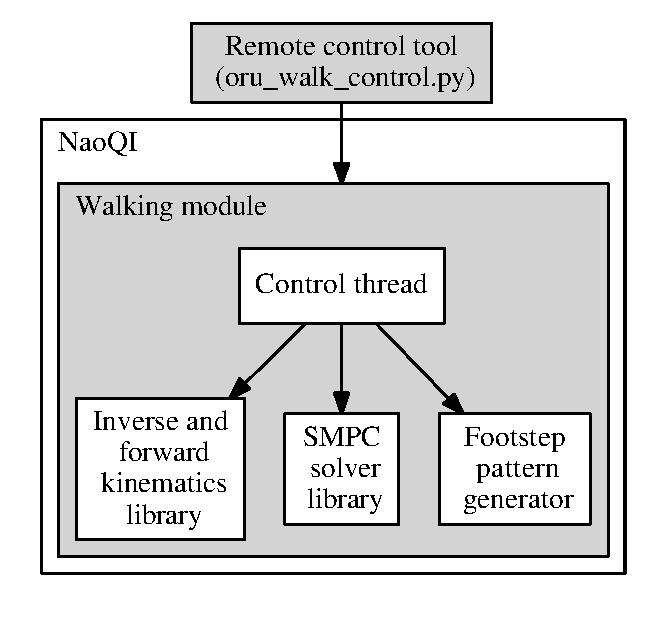
\includegraphics[scale=0.6]{Figures/nao_mod_arch.eps}}
    \caption{Architecture of the walking module}
    \label{fig.arch}
\end{figure}

The walking module runs within the \verb|NaoQI| framework on a Nao robot. Commands 
are sent to the module using a simple command line control tool from a personal 
computer.

When walk is started the module reads parameters from a configuration file and
spawns a control thread, which is periodically activated in order to determine
the joint commands. The necessary joint angles are determined based on the 
desired position of the \ac{CoM} and poses of the feet provided by \ac{MPCWMG}
solvers and footstep pattern generator, respectively. The functions of each submodule
are described in more detail in this chapter.

Note that some implementations \cite{NaoWalk} assume that the \ac{CoM} is fixed to 
the torso, hence the trajectory of the \ac{CoM} is tracked by some point on the
torso. We do not make such assumption and control the real \ac{CoM}.



%%%%%%%%%%%%%%%%%%%%%%%%%%%%%%%%%%%%%%%%%%%%%%%%%%%%%%%%%%%%%%%%%%%%%%%%%%%%%%%%%%
%%%%%%%%%%%%%%%%%%%%%%%%%%%%%%%%%%%%%%%%%%%%%%%%%%%%%%%%%%%%%%%%%%%%%%%%%%%%%%%%%%
%%%%%%%%%%%%%%%%%%%%%%%%%%%%%%%%%%%%%%%%%%%%%%%%%%%%%%%%%%%%%%%%%%%%%%%%%%%%%%%%%%
\section{Sparse MPC Solver}
The purpose of the \ac{MPCWMG} is to generate a trajectory for the \ac{CoM}. To be
precise, a trajectory for the \ac{ZMP} is generated first, then the \ac{CoM}
positions are computed from it. The trajectories are shown in \cref{fig.footsteps}.
In order to generate trajectories the reference \ac{ZMP} points must be given,
in \ac{SS} they are placed in the middle of the constraining rectangle, in a \ac{DS} 
the reference \ac{ZMP} point of the closest \ac{SS} is used.

\begin{figure}[ht]
    \centerline{%
    \includegraphics[scale=0.5]{Figures/sim_nodist_as.eps}}
    \caption[Footsteps and trajectories of {\bf CoM} and {\bf ZMP}]{Red and black rectangles
    represent \ac{SS}, \ac{DS} are omitted. Blue and black curves show trajectories 
    of \ac{CoM} and \ac{ZMP}, respectively. Black circles stand for reference 
    \ac{ZMP} positions. Green boxes are the footstep reference points. The data was obtained
    during simulation.}
    \label{fig.footsteps}
\end{figure}

Both active set (\cref{sec.as}) and logarithmic barrier (\cref{sec.ip}) 
methods were developed for solving the \ac{QP}. One of them can be 
selected by appropriately setting options in the configuration file. In particular,
these options can be used to control the mechanisms that limit the execution
time of the solver. The execution time of active set method can be controlled 
by imposing a limit on the number of activated constraints and disabling the 
deactivation of constraints. The number of iterations of the logarithmic barrier
method can be also explicitly limited.


%%%%%%%%%%%%%%%%%%%%%%%%%%%%%%%%%%%%%%%%%%%%%%%%%%%%%%%%%%%%%%%%%%%%%%%%%%%%%%%%%%
%%%%%%%%%%%%%%%%%%%%%%%%%%%%%%%%%%%%%%%%%%%%%%%%%%%%%%%%%%%%%%%%%%%%%%%%%%%%%%%%%%
%%%%%%%%%%%%%%%%%%%%%%%%%%%%%%%%%%%%%%%%%%%%%%%%%%%%%%%%%%%%%%%%%%%%%%%%%%%%%%%%%%
\section{Footstep Pattern Generator}
The functionality of the footstep pattern generator is two-fold. It provides
functions to predefine footsteps and generate swing foot trajectories during 
walk.

The positions and orientations of the footsteps must be defined before walk is
started, an example of footstep sequence is depicted in \cref{fig.footsteps}. 
% Automatic footstep generation was left out of the scope of this thesis. TODO

\begin{figure}[ht]
    \centerline{%
    \includegraphics[scale=0.5]{Figures/foottraj.eps}}
    \caption[Swing foot trajectory]{Right swing foot trajectory in three
    projections. Red crosses show points that correspond to sampling intervals
    of $20$ milliseconds. The data was obtained during simulation.}
    \label{fig.foottraj}
\end{figure}

The foot trajectories are generated using Bezier curves. Parameters for the curves
were found experimentally. The three projections of a right foot trajectory produced
during straight walk are shown in \cref{fig.foottraj}, the trajectory of the left 
foot is symmetric.



%%%%%%%%%%%%%%%%%%%%%%%%%%%%%%%%%%%%%%%%%%%%%%%%%%%%%%%%%%%%%%%%%%%%%%%%%%%%%%%%%%
%%%%%%%%%%%%%%%%%%%%%%%%%%%%%%%%%%%%%%%%%%%%%%%%%%%%%%%%%%%%%%%%%%%%%%%%%%%%%%%%%%
%%%%%%%%%%%%%%%%%%%%%%%%%%%%%%%%%%%%%%%%%%%%%%%%%%%%%%%%%%%%%%%%%%%%%%%%%%%%%%%%%%
\section{Inverse and Forward Kinematics Library}\label{sec.ik}
Inverse and forward kinematics library provide functions that solve \ac{FK} and \ac{IK}.
In the sources it is also referred to as \ac{IGM}, where the word ``geometrical'' is used 
instead of ``kinematics'' to emphasize, that the library works with positions of actuators 
and not with their motions.


%%%%%%%%%%%%%%%%%%%%%%%%%%%%%%%%%%%%%%%%%%%%%%%%%%%%%%%%%%%%%%%%%%%%%%%%%%%%%%%%%%
\subsection{Algorithms}\label{sec.ik_alg}
From a mechanical point of view a humanoid robot is a chain of $n+1$ rigid bodies
({\bf links}) connected by $n$ {\bf joints}. One of the extremities of this chain 
is often referred to as the base and some of the others as end-effectors. Motions 
of a robot are compositions of elementary motions of links with respect to each 
other. Motion can be represented in two spaces: {\bf joint space} and {\bf operational 
space}, in the former one the coordinates are $n$ joint angles, in the latter -- 
positions and orientations of end-effectors with respect to the base. Joint and 
operational spaces are related by \ac{FK} and \ac{IK}.

Let $\mbm{q} \in \RR^n$ be the joint space coordinates, and $\mbm{r} \in \RR^m$ be 
the operational space coordinates.

The purpose of the \ac{FK} is determination of position and orientation 
of a frame attached to an end-effector given the reference frame attached to the base
of the chain and a set of joint angles. It is performed by solving
$$
\mbm{r} = f_r(\mbm{q}).
$$

The \ac{IK} problem is opposite to the \ac{FK} problem. \ac{IK} finds the set of joint 
angles that realizes the desired pose of an end-effector using inverse function of $f_r$
$$
\mbm{q}=f_r^{-1}(\mbm{r}).
$$

There are two approaches to solve the \ac{IK} problem: analytical (closed-form) and 
numerical. The \ac{IK} is a typical nonlinear problem and it is not always possible to 
find a closed-form solution. In such cases numerical methods can be used instead.
A numerical solution of \ac{IK} can be found in a several ways using different iterative
schemes. The implementation of \ac{IK} for Nao used in our work is similar to the method 
described in \cite{ZhangIKRep}.

The Taylor approximation of the \ac{FK} function can be expressed as
\begin{equation}\label{eq.ik_taylor}
\mbm{r} = f_r(\mbm{q}) \approx f_r(\mbm{q}_k) + \mbm{J}_r(\mbm{q}_k)(\mbm{q}-\mbm{q}_k),
\end{equation}
%
where $\mbm{q}_k$ is the initial approximation of the solution, and $\mbm{J}_r$ is the
$m \times n$ Jacobian matrix, whose computation is described in detail in 
\cite{AntonioThesis}. Let $\mbm{e}_r = \mbm{r} - f_r(\mbm{q}) = f_r(\mbm{q}_k)$ 
and $\Delta\mbm{q} = \mbm{q}-\mbm{q}_k$, then from \cref{eq.ik_taylor} we obtain
%
\begin{equation}\label{eq.ik_eqc}
\mbm{e}_r = \mbm{J}_r(\mbm{q}_k)\Delta\mbm{q},
\end{equation}

Consider the optimization problem
\begin{equation}\label{eq.ik_opt}
\begin{split}
\minimize{\Delta\mbm{q} \in \mathbb{R}^n} 
            & \frac{1}{2} \norm{ \Delta\mbm{q} + \mbm{e}_q}^2_{\mbm{H}} \\
\subjectto  & \mbm{e}_r = \mbm{J}_r(\mbm{q}_k)\Delta\mbm{q},
\end{split}
\end{equation}
where $\mbm{e}_q = \mu_{ik} (\mbm{q}_k - \mbm{q}_0)$ is the weighted difference between the 
initial guess and the reference joint angles $\mbm{q}_0$. $\mbm{e}_q$ is added to the 
objective function in order to obtain repetitive solutions.

The optimization problem~\eqref{eq.ik_opt} is equivalent to
\begin{equation}\label{eq.ik_opt_final}
\begin{split}
\minimize{\Delta\mbm{q} \in \mathbb{R}^n} 
            & \frac{1}{2} \norm{ \Delta\mbm{q} }^2_{\mbm{H}} + \mbm{e}_q^T \mbm{H} \Delta\mbm{q} \\
\subjectto  & \mbm{e}_r = \mbm{J}_r(\mbm{q}_k)\Delta\mbm{q}.
\end{split}
\end{equation}



%%%%%%%%%%%%%%%%%%%%%%%%%%%%%%%%%%%%%%%%%%%%%%%%%%%%%%%%%%%%%%%%%%%%%%%%%%%%%%%%%%
\subsection{Implementation}
The support foot is selected as the fixed base of the kinematic tree. Consequently,
the base must be periodically changed. This change is performed in the end of \ac{DS}
and is a source of error, that must be accounted for (see Section 
\cref{sec.err_feedback}). In theory, it is possible to always use the same foot as 
the base assuming that the position tracking for this foot is perfect, but this 
assumption is admissible only in simulation. 

Alternatively, the torso can be selected as the base \cite{NaoWalk}. Due to implicit
error feedback it might a better choice when a robot is subject to disturbances.
%For example, consider a situation when a robot is held back by a wall. If 
%one foot is chosen as the base, the robot tries to bring the \ac{CoM} through the 
%wall and fails. On the other hand, if the torso is the base, then 

The functions that solve \ac{FK}, compute the Jacobian $\mbm{J}_r$ and $\mbm{e}_r$
were generated using \verb|Maple|\footnote{The code is available as well 
at \url{https://github.com/asherikov/}.}. 

Two \ac{FK} functions are used. The first one determines pose of a swing foot, when 
change of the base is performed. The second computes the \ac{CoM} position for error 
feedback.
%, it requires knowledge of the poses and \ac{CoM}s of all links is necessary.

The \ac{QP}~\eqref{eq.ik_opt_final} is solved using block elimination with $\mbm{H} = 
\mbm{I}$, and $\mu_{ik}$ was determined experimentally. The problem is resolved until 
the change in joint angles becomes smaller than the minimal angle detected by the 
joint position sensors. Also, a limit on the number of iterations is imposed to 
detect cases, when there is no solution.

\begin{figure}[ht]
    \centerline{%
    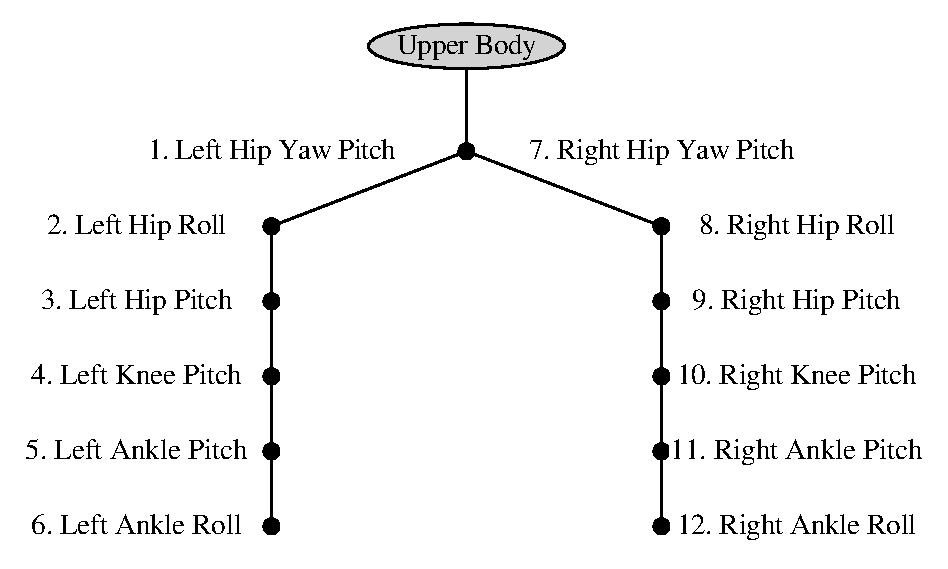
\includegraphics[scale=0.6]{Figures/nao_joints.eps}}
    \caption{Lower body joints of Nao}
    \label{fig.joints}
\end{figure}

The joint angles of the upper body are fixed, hence only $12$ lower body joints depicted 
in \cref{fig.joints} are controlled. Note that joints $1$ and $7$ are coupled
\footnote{Refer to \url{http://www.aldebaran-robotics.com/documentation/index.html} for
more information.}, that is, they share the same motor and move simultaneously and 
symmetrically. In the case of conflicting orders \verb|LHipYawPitch| always takes priority. 
The coupling between these joints is handled by imposing an equality constraint 
$\Delta\mbm{q}_1 = \Delta\mbm{q}_7$. It is also possible to reduce the number of controlled 
joints to account for this. 

The total number of imposed constraints is $10$:
\begin{itemize}
    \item $3$ on the position of the swing foot;
    \item $3$ on the orientation of the swing foot;
    \item $3$ on the position of the \ac{CoM};
    \item $1$ to take into account the coupled joint.
\end{itemize}

Several alternative versions of \ac{IK} implementation were also tested. In the early 
variants of the \ac{IK} module the difference between the joint angles and the reference 
angles is not penalized, but the constraints on the orientation of the frame fixed to 
the \ac{CoM} are used instead. These constraints are imposed in such a way, that the 
rotation about $x$ and $y$ axes is not allowed. The constraint on rotation about $x$ 
axis was removed in order to reduce the load on the \verb|HipRoll| joints, which tend 
to violate their limits for some \ac{CoM} trajectories otherwise. Further experiments 
demonstrated, that the gait is better, when there are no constraints on the orientation 
of the \ac{CoM}. Also, it is unclear how to define the desired orientation of the \ac{CoM} 
in a general case, for example, during a circular walk. The penalization of the 
difference with the reference joint angles was introduced to maintain upright posture
and avoid failures due to bad configurations of the lower body joints.

Another version of \ac{IK} is similar to the current one, but it controls all joints of 
the robot instead of only the lower body joints. However, the ability to cope with external 
disturbances is roughly the same. Furthermore, this approach requires more time for 
computations.

%It is assumed that the leading matrix of the constraints is nonsingular.



%%%%%%%%%%%%%%%%%%%%%%%%%%%%%%%%%%%%%%%%%%%%%%%%%%%%%%%%%%%%%%%%%%%%%%%%%%%%%%%%%%
%%%%%%%%%%%%%%%%%%%%%%%%%%%%%%%%%%%%%%%%%%%%%%%%%%%%%%%%%%%%%%%%%%%%%%%%%%%%%%%%%%
%%%%%%%%%%%%%%%%%%%%%%%%%%%%%%%%%%%%%%%%%%%%%%%%%%%%%%%%%%%%%%%%%%%%%%%%%%%%%%%%%%
\section{Control Thread}
The logic of one control loop of the control thread is shown in \cref{fig.seq}. 

\begin{figure}[ht]
    \centerline{%
    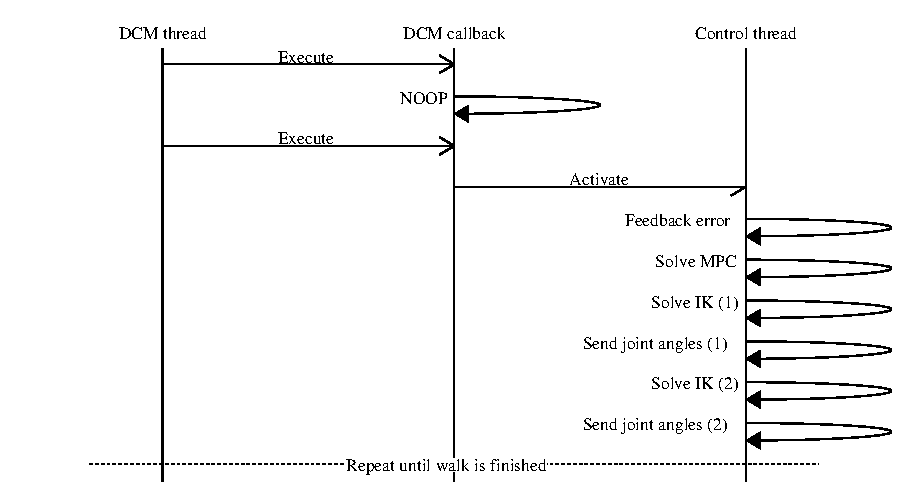
\includegraphics[scale=0.8]{Figures/nao_mod_seq.eps}}
    \caption{Control loop of the walking module}
    \label{fig.seq}
\end{figure}


%%%%%%%%%%%%%%%%%%%%%%%%%%%%%%%%%%%%%%%%%%%%%%%%%%%%%%%%%%%%%%%%%%%%%%%%%%%%%%%%%%
\subsection{Real-time Control Features of the Nao API}
The control of a walking robot must be performed in real-time. \ac{API} of a Nao
robots provides two possible ways to implement this. The first one is to register 
callback function from \ac{DCM}, which is activated each $10$ milliseconds. The main
purpose of the \ac{DCM} is to update sensor readings in the memory, since there is
no direct access to the sensors. The second way is to register callback function 
from the built-in \verb|Motion| module, which is activated each $20$ milliseconds. 
The \verb|Motion| module can perform walk and other operations, but it is activated
even if no commands were sent. 

We have tried to use both methods for real-time control. Experiments have 
demonstrated, that period of $10$ milliseconds is too short to perform all necessary 
operations. On the other hand, when the callback from \verb|Motion| module was
used, it was observed, that the sensor readings are not necessary updated twice
during the $20$ milliseconds between activations of the module (at least in the
simulation on a personal computer). Hence, a control thread was introduced, which 
is activated by a callback function that is called when \ac{DCM} finishes its work. 
Thus the callback function is executed each $10$ milliseconds. It has a counter of 
executions, and on each even execution (that is, each $20$ milliseconds) it wakes up 
the control thread using a synchronization tool provided by the \verb|Boost| library. 

The priority of the control thread plays a critical role, since sometimes it is not 
possible to complete all necessary computations in available time using the default 
priority. We use \verb|SCHED_FIFO| scheduling policy, the same as \ac{DCM} thread 
uses. The priority is set to $65$. Note that \verb|NaoQi| does not run with root 
privileges and priority cannot be set arbitrarily. 


%%%%%%%%%%%%%%%%%%%%%%%%%%%%%%%%%%%%%%%%%%%%%%%%%%%%%%%%%%%%%%%%%%%%%%%%%%%%%%%%%%
\subsection{Error Feedback}\label{sec.err_feedback}
On the feedback step the position of the \ac{CoM} is computed based on the current
joint angles. Then the error between the computed and the expected positions of
the \ac{CoM} is computed. The expected position is taken from the previous solution
of \ac{MPCWMG}. If the error is below a given threshold, it is silently discarded,
otherwise it is scaled by a gain and added to the expected position of the \ac{CoM}. 
Error feedback for the velocity and acceleration of the \ac{CoM} is not performed. 
The state obtained after error feedback is used as initial state of the \ac{MPCWMG}.

There is also a second type of error feedback, which is performed when the reference
foot is changed. Note that when the new reference foot touches the ground its position
is not exactly the same as the target one. Therefore, if the reference frame is
moved to this foot, an error in position of \ac{CoM} appears. To avoid this effect the
footstep pattern generator is informed about the error in foot position before the
reference foot is changed. It is also necessary to synchronize joint angles in the 
model of the robot, which is used in inverse kinematics library, with the joint angles 
obtained from sensors.


%%%%%%%%%%%%%%%%%%%%%%%%%%%%%%%%%%%%%%%%%%%%%%%%%%%%%%%%%%%%%%%%%%%%%%%%%%%%%%%%%%
\subsection{Accounting for the Computational Delay}\label{sec.mpc_delay}
Quadratic programming is a time demanding task, and it takes a considerable part of 
one control sampling period. It is impossible to obtain smooth joint motions without 
accounting for the computational delay. The model of the system can be modified for 
this purpose as described in Section $2.5$ of \cite{MacMPC}. However, for the sake 
of simplicity the system was not modified, and a heuristic described in this section 
was used instead.

The simplest workaround is to continue execution of the commands obtained on the 
previous iteration until the new commands are available. On the other hand, if the 
old commands are not finished before the start of the next iteration, it might be
difficult to perform error feedback, since it is necessary to have a good estimation
of the desired state. The last problem can be addressed by solving the \ac{IK} twice,
so that there are two sets of commands: one must be executed in one control sampling
period and the second one is used, while the new solution is not available. The joint 
angles from the second set are expected to be reached in two control sampling periods. 
As soon as the first solution of inverse kinematics is obtained the commands are sent
to the joint controllers to replace the commands sent on the previous iteration. It
takes $1$ millisecond for joint controllers to react to the new commands. Note that 
the second \ac{IK} solution can be used as initial guess for the first \ac{IK} in the 
next control loop leading to a smaller number of \ac{IK} iterations.

In some situations the computation time may exceed the time available for one
iteration of the control loop, such situations are potentially dangerous and
must be avoided. In order to enforce the time limits, a simple mechanism was 
developed that interrupts the execution of the walk, if the duration of one 
iteration of the control loop exceeded $15$ milliseconds.

%-------------------------------------------------------------------------------
\chapter{Experimental Results}
\label{ch.results}
%-------------------------------------------------------------------------------
%\cite{FastMPC}
%\cite{BartlettASvsIP}
%\cite{FerreauASWarm}
%\cite{RaoIPMPC}

This chapter describes the results of the experiments, which were conducted on 
a robot and in a simulation on a personal computer. The experiments on a robot
were performed in order to evaluate and tune the control scheme as a whole.
The comparison of the active set and logarithmic barrier solvers was also
performed in simulation, since there are too many factors that can affect 
the performance on a robot, and it is rather difficult to apply disturbances to 
a robot in a repeatable manner. Note that even in the simulation it is necessary
to check the feasibility of the generated \ac{CoM} trajectory using the inverse
kinematics module. 

The results of the tests presented in this chapter were obtained during a straight 
walk. However, the walking module can realize more complex patterns, for example,
circular walk\footnote{Video recordings of walk patterns realized by our control
module can be accessed at \url{http://www.youtube.com/playlist?list=PL93B16B2910EC7F3D&feature=plcp}}.



%%%%%%%%%%%%%%%%%%%%%%%%%%%%%%%%%%%%%%%%%%%%%%%%%%%%%%%%%%%%%%%%%%%%%%%%%%%%%%%%
%%%%%%%%%%%%%%%%%%%%%%%%%%%%%%%%%%%%%%%%%%%%%%%%%%%%%%%%%%%%%%%%%%%%%%%%%%%%%%%%
%%%%%%%%%%%%%%%%%%%%%%%%%%%%%%%%%%%%%%%%%%%%%%%%%%%%%%%%%%%%%%%%%%%%%%%%%%%%%%%%
\section{Parameters of the Walk and Quadratic Problem}\label{sec.parameters}
The walk is affected by a number of parameters. Some of them were preset, while
others were tuned during experiments on a robot. 

The step height and length were set beforehand. The height of the step is $2$ 
centimeter. The step length is controlled by a parameter, which specifies the 
displacement of a footstep with respect to the previous footstep along the $x$ 
axis. This parameter is equal to $4$ centimeter, hence, the full step length
is $8$ centimeter. 

The parameters of Bezier curves that are used to generate foot trajectories were
found using trial and error approach. The trajectory is shown in \cref{fig.foottraj}.

The length of one \ac{SS} phase is set to $400$ millisecond. The \ac{DS} phase
takes $120$ millisecond and is approximated by $3$ ``fake'' \ac{DS} with rectangular
constraints as described in \cref{sec.ds_constraints}.

The preview window includes $40$ sampling intervals. The first two sampling
intervals are set to $20$ millisecond, since we use the first two states from
the solution of \ac{MPCWMG} (see \cref{sec.mpc_delay} for more information).
The default time for the remaining sampling intervals is $40$ millisecond 
in order to obtain a longer preview window as explained in \cref{sec.timevarsys}.
However, sometimes it is not possible to set all remaining intervals to $40$
millisecond and one of them must be also set to $20$ millisecond. For example,
if one iteration of the control loop is spent in \ac{SS}, the remaining time in
this \ac{SS} is $380$ millisecond, which cannot be divided into intervals of $40$
millisecond. Thus, the total length of the preview window is $2*20 + 38*40 = 1560$ 
or $2*20 + 37*40 + 20 = 1540$ millisecond. 

It is possible to increase the default length of a preview interval, but it has 
negative effects on the gait. Also, the length of all sampling intervals in the
preview window can be set to $20$ millisecond. In this case if the number of 
sampling intervals is not changed, the length of a preview window is significantly 
shorter and a robot does not compensate for external disturbances as well. On the 
other hand, if the number of sampling intervals is increased, a solution of a 
bigger \ac{QP} problem takes more time.

The parameter $\mu_{ik}$, which penalizes the difference with the reference joint
angles in the inverse kinematics \ac{QP} (\cref{sec.ik_alg}), is set to $1.2$.

The gain and threshold for error feedback of \ac{CoM} position are set to $0.3$ 
and $4$ millimeters. The purpose of these parameters is described in 
\cref{sec.err_feedback}. If the threshold is high, the compensation for external
disturbances is not sufficient. 

The solutions of \ac{MPCWMG} are affected by four gains. The first one $\alpha_g$ 
penalizes the difference between the computed \ac{ZMP} trajectory and reference 
\ac{ZMP} points. The last three $\beta_g, \gamma_g, \eta_g$ penalize the absolute
values of velocity, acceleration, and jerk of the \ac{CoM}. It was observed, that 
$\alpha_g$ is the most important. The values of the gains are $\alpha_g = 8000$,
$\beta_g = \gamma_g = \eta_g = 1$. If $\alpha_g$ is set to a smaller value, the 
threshold for \ac{CoM} error feedback must be increased to avoid generation of 
infeasible \ac{CoM} trajectories. 



%%%%%%%%%%%%%%%%%%%%%%%%%%%%%%%%%%%%%%%%%%%%%%%%%%%%%%%%%%%%%%%%%%%%%%%%%%%%%%%%
%%%%%%%%%%%%%%%%%%%%%%%%%%%%%%%%%%%%%%%%%%%%%%%%%%%%%%%%%%%%%%%%%%%%%%%%%%%%%%%%
%%%%%%%%%%%%%%%%%%%%%%%%%%%%%%%%%%%%%%%%%%%%%%%%%%%%%%%%%%%%%%%%%%%%%%%%%%%%%%%%
\section{Experiments on a Robot}
The purpose of the experiments conducted on a Nao robot was to evaluate quality
of the produced gait, compare the two developed \ac{MPCWMG} solvers, and identify
potential improvements of the control scheme.

Initial tuning of the parameters of the walking module was performed using the active
set method. Then the parameters of the logarithmic barrier method were found. The 
approximate solution of the \ac{QP} by logarithmic barrier method does not have
negative effects on the gait (see \cref{fig.com_xy,fig.com_error}).

\begin{figure}[!ht]
    \centering
    \subfigure[\acs{MPCWMG} is solved using the active set method]{
    \includegraphics[scale=0.5]{Figures/as_com_xy.eps}}
    \subfigure[\acs{MPCWMG} is solved using the logarithmic barrier method]{
    \includegraphics[scale=0.5]{Figures/ip_com_xy.eps}}
\caption[Footsteps and projection of {\bf CoM} trajectory to $x\mbox{-}y$ plane]{The 
footsteps and projection of \acs{CoM} to $x\mbox{-}y$ plane. The data is gathered 
during execution of a walking module on a robot. Red and black rectangles show 
positions of the footsteps. \ac{CoM} trajectory generated by the solver is 
represented by the blue curve. The red line shows the measured position of 
\ac{CoM}.}
\label{fig.com_xy}
\end{figure}

During the straight walk the active set method does not deactivate constraints,
the maximal number of added constraints is $7$. In the initial and final double 
supports constraints are not added, during the walk the number of activated 
constraints is usually 6 or 7. The parameters of the logarithmic barrier method 
were selected in such a way that it makes only one iteration of the external 
loop, then the number of internal loops was limited to $3$.

\begin{table}
\begin{center}
\begin{tabular}{c|p{1.5cm}|p{2.5cm}||p{1.5cm}|p{2.5cm}}
            & \multicolumn{2}{c||}{Total time (second)}  & \multicolumn{2}{c}{Solution of the \acs{QP} (second)}\\
\hline
            & Active set method & Logarithmic barrier method & Active set method & Logarithmic barrier method \\
\hline
    minimal & $0.001867$  &   $0.004108$                    & $0.000490$  &   $0.002569$                    \\
    mean    & $0.003071$  &   $0.004834$                    & $0.001259$  &   $0.003016$                    \\
    maximal & $0.004650$  &   $0.006012$                    & $0.002782$  &   $0.004126$                    \\
\end{tabular}
\caption[Execution time of the control loop]{
The amount of time spent in one iteration of the control loop and fraction of this time consumed by the solvers.}
\label{tbl.time}
\end{center}
\end{table}

\begin{figure}[ht]
    \centerline{%
    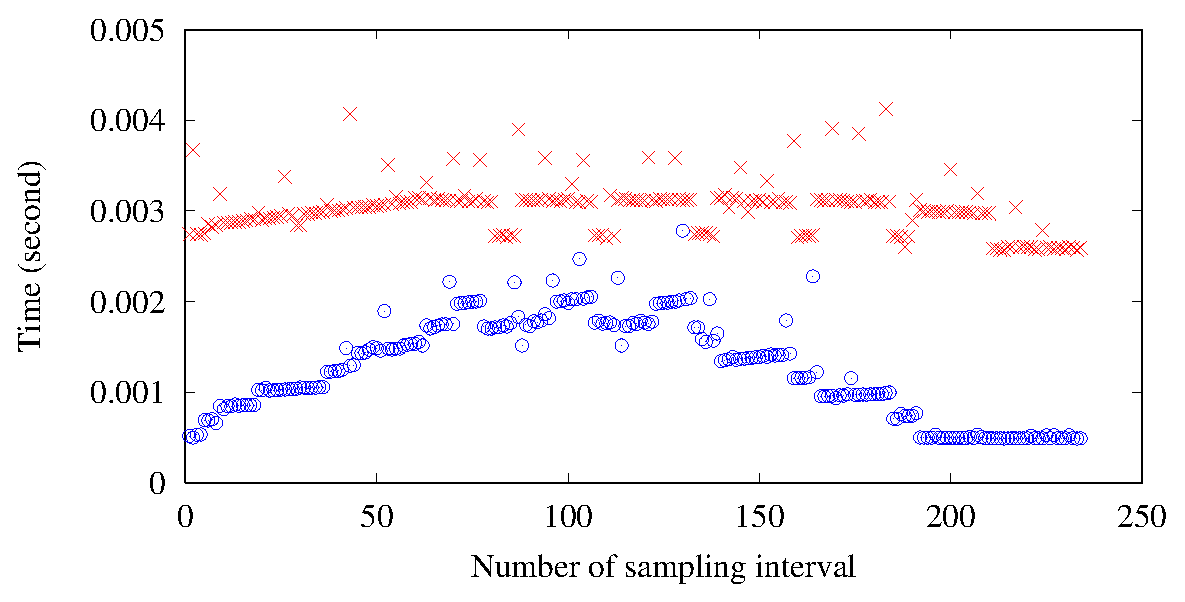
\includegraphics[scale=0.5]{Figures/qp_time.eps}}
    \caption[Execution time of the solvers]{Execution time of the solvers on a robot during
    a straight walk. The red crosses show execution time of the logarithmic barrier method,
    the blue circles -- the active set method.}
    \label{fig.qp_time}
\end{figure}

Measurements of the execution time are presented in \cref{tbl.time} and in 
\cref{fig.qp_time}. The total execution time includes logging, which takes about 
$0.0005$ second, solution of the \ac{MPCWMG} problem, and solution of two inverse 
kinematics problems. The solution of one inverse kinematics problem takes from 
$1$ to $4$ iterations, in $80$\% of cases the number of iterations is not bigger 
than $2$.

\begin{figure}[!ht]
    \centering
%\begin{minipage}[t]{0.48\linewidth}
    \subfigure[Trajectory of the left foot]{
    \includegraphics[scale=0.5]{Figures/left_foot_traj.eps}}
%\end{minipage}
%\hspace{\fill}
%\begin{minipage}[t]{0.48\linewidth}
    \subfigure[Trajectory of the right foot]{
    \includegraphics[scale=0.5]{Figures/right_foot_traj.eps}}
%\end{minipage}
\caption[Foot trajectory tracking]{Tracking of the foot trajectories in $x\mbox{-}z$
plane. The blue line is the trajectory generated using Bezier curve, the red one 
shows the position of the foot computed by forward kinematics function based on the 
measured joint angles.}
\label{fig.robot_foottraj}
\end{figure}

The generated foot trajectories are not followed precisely, due to the action 
of gravity on the swing foot, see \cref{fig.robot_foottraj}. Note that
the right foot does not track the desired trajectory as well as the left.
This effect persists, if the walk is started from different leg. One of the
possible reasons is a flaw of the hardware of the robot, which was used for tests. 

\begin{figure}[ht]
    \centerline{%
    \includegraphics[scale=0.5]{Figures/hiproll.eps}}
    \caption[Joint trajectory tracking]{Tracking of the right hip roll joint trajectory
    produced by the inverse kinematics module. The blue curve is the generated trajectory,
    while the red one shows the measured joint angle.}
    \label{fig.hiproll}
\end{figure}

There is also an error in tracking of joint trajectories, an example is given in
\cref{fig.hiproll}. Several factors cause this error: action of the gravity, 
infeasible joint velocities, and the delay in sensor readings. It is desirable
to account for some of these factors to improve the performance of the walking
module.

\begin{figure}[!ht]
    \centering
%\begin{minipage}[t]{0.48\linewidth}
    \subfigure[Projection of {\bf CoM} trajectory to $x\mbox{-}z$ plane]{
    \includegraphics[scale=0.5]{Figures/as_com_xz.eps}}
%\end{minipage}
%\hspace{\fill}
%\begin{minipage}[t]{0.48\linewidth}
    \subfigure[Projection of {\bf CoM} trajectory to $y\mbox{-}z$ plane]{
    \includegraphics[scale=0.5]{Figures/as_com_yz.eps}}
%\end{minipage}
\caption[Projections of {\bf CoM} trajectory to $x\mbox{-}z$ and $y\mbox{-}z$ planes]{
Projections of \acs{CoM} trajectory generated using the active set method to $x\mbox{-}z$ 
and $y\mbox{-}z$ planes. The data is gathered during execution of a walking module on 
a robot. The reference height of \ac{CoM}, which is always constant, is represented by 
the blue line. The red curve shows the measured position of \ac{CoM}.}
\label{fig.com_xyz}
\end{figure}

\begin{figure}[!ht]
    \centering
%\begin{minipage}[t]{0.48\linewidth}
    \subfigure[\acs{MPCWMG} is solved using the active set method]{
    \includegraphics[scale=0.5]{Figures/as_com_error.eps}}
%\end{minipage}
%\hspace{\fill}
%\begin{minipage}[t]{0.48\linewidth}
    \subfigure[\acs{MPCWMG} is solved using the logarithmic barrier method]{
    \includegraphics[scale=0.5]{Figures/ip_com_error.eps}}
%\end{minipage}
\caption[Error in {\bf CoM} position]{Error in \ac{CoM} position. Blue, red, 
and black lines correspond to error along $x$, $y$, and $z$ axes, respectively.}
\label{fig.com_error}
\end{figure}

Due to the errors in tracking of foot and joint trajectories and, probably,
other factors, a significant error in \ac{CoM} appears (see 
\cref{fig.com_xy,fig.com_xyz,fig.com_error}). The performance heavily depends 
on the error feedback. If the error feedback is disabled by setting the 
respective gain to zero, the robot starts to wobble after a few steps and 
soon falls.

It was mentioned in \cref{sec.err_feedback}, that there is a second type of 
error feedback, which corrects the positions of footsteps. The result of this
feedback can be clearly seen in \cref{fig.com_xy}, when compared to the 
footsteps obtained in simulation that are shown in \cref{fig.footsteps}.



%%%%%%%%%%%%%%%%%%%%%%%%%%%%%%%%%%%%%%%%%%%%%%%%%%%%%%%%%%%%%%%%%%%%%%%%%%%%%%%%
%%%%%%%%%%%%%%%%%%%%%%%%%%%%%%%%%%%%%%%%%%%%%%%%%%%%%%%%%%%%%%%%%%%%%%%%%%%%%%%%
%%%%%%%%%%%%%%%%%%%%%%%%%%%%%%%%%%%%%%%%%%%%%%%%%%%%%%%%%%%%%%%%%%%%%%%%%%%%%%%%
\section{Experiments in a Simulation}
One of the goals of the thesis is to compare active set and logarithmic barrier
methods for solution of \ac{MPCWMG}. Comparison of these methods in the presence
of external disturbances on a robot is complicated due to the necessity to apply such
disturbances in a repeatable manner. Hence, some of the tests were performed
during simulation of the walk on a personal computer. The \ac{CoM} trajectories 
were generated with the same parameters as on the robot. The inverse kinematics 
module was adopted to ensure feasibility of these trajectories, since neither 
optimality or stability of \ac{MPCWMG} solutions imply feasibility (see 
\cref{fig.sim_dist}).

The \ac{CoM} trajectories that were obtained in the simulation without any 
disturbances are shown in \cref{fig.sim_nodist}.

\begin{figure}[!ht]
    \centering
%\begin{minipage}[t]{0.48\linewidth}
    \subfigure[Trajectory generated using the active set method]{
    \includegraphics[scale=0.5]{Figures/sim_nodist_as.eps}}
%\end{minipage}
%\hspace{\fill}
%\begin{minipage}[t]{0.48\linewidth}
    \subfigure[Trajectory generated using the logarithmic barrier method]{
    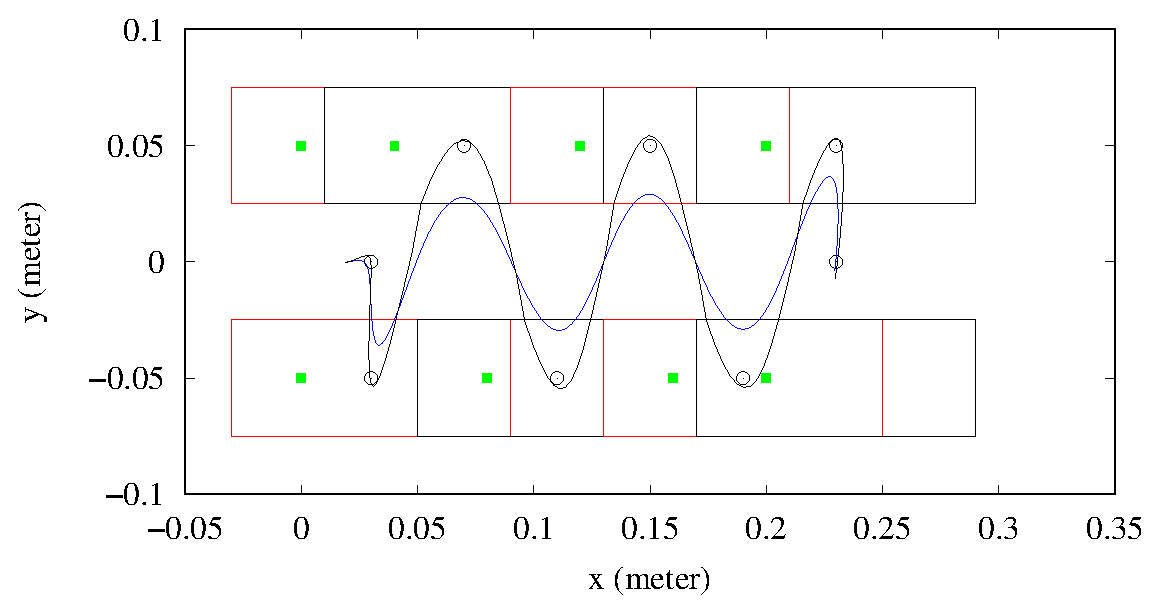
\includegraphics[scale=0.5]{Figures/sim_nodist_ip.eps}}
%\end{minipage}
\caption[Trajectories of {\bf CoM} in a simulation]{Trajectories of {\bf CoM} in a 
simulation. Red and black rectangles represent \ac{SS}, \ac{DS} are omitted. Blue 
and black curves show trajectories of \ac{CoM} and \ac{ZMP}, respectively. Black 
circles stand for reference \ac{ZMP} positions. Green boxes are the footstep 
reference points.}
\label{fig.sim_nodist}
\end{figure}

The disturbances are applied by instantaneous change of the position of \ac{CoM} 
to replicate error feedback on the robot. An example is shown in \cref{fig.sim_dist}. 
During one simulation run the system is disturbed only once. The displacement of
\ac{CoM} is no more than two centimeters along one of the axes in the horizontal
plane. 

It was observed that strong disturbances (more than one centimeter) often lead to 
instability of the \ac{MPCWMG}, when the \ac{CoM} trajectory diverges. 

\begin{figure}[!ht]
    \centering
%\begin{minipage}[t]{0.48\linewidth}
    \subfigure[Trajectory generated using the active set method]{
    \includegraphics[scale=0.5]{Figures/sim_infeas_as.eps}}
%\end{minipage}
%\hspace{\fill}
%\begin{minipage}[t]{0.48\linewidth}
    \subfigure[Trajectory generated using the logarithmic barrier method]{
    \includegraphics[scale=0.5]{Figures/sim_infeas_ip.eps}}
%\end{minipage}
\caption[Trajectories of {\bf CoM} in the presence of disturbance]{Trajectories of 
{\bf CoM} in the presence of disturbance. Red and black rectangles represent \ac{SS}, 
\ac{DS} are omitted. Blue and black curves show trajectories of \ac{CoM} and \ac{ZMP}, 
respectively. Black circles stand for reference \ac{ZMP} positions. Green boxes are 
the footstep reference points. The red stars indicate infeasible \ac{CoM} positions.}
\label{fig.sim_dist}
\end{figure}

The disturbances have a strong effect on the performance of the active set method, since
the number of constraints at the optimal point is often higher. In some situations the size
of the active set reaches $40$, which makes the solution computationally infeasible on a 
robot. In order to enforce the time limits, the deactivation of constraints can be disabled 
and the maximal number of activated constraints can be fixed. If the limit on the number 
of the activated constraints is relatively high (bigger than $20$), the approximate solution 
is often admissible. However, strict limits, as well as disabled deactivation of constraints
may lead to instability.

\begin{figure}[ht]
    \centerline{%
    \includegraphics[scale=0.5]{Figures/obj_asip.eps}}
    \caption[The decrease rate of objective function]{The decrease rate of objective 
    function. The values produced using active set and logarithmic barrier method 
    are represented by the blue and red lines, respectively.}
    \label{fig.obj_asip}
\end{figure}

The \ac{MPCWMG} may also become unstable, if there are no disturbances, but a rather 
strict limit on the number of active constraints is imposed. The properly tuned
logarithmic barrier method can be safer in this case, since it results in higher 
decrease rate of the value of the objective function (see \cref{fig.obj_asip})
in the number of iterations.

%-------------------------------------------------------------------------------
\chapter{Conclusion}
\label{ch.conclusion}
%-------------------------------------------------------------------------------
A short summary of the work presented in the thesis is given in this chapter. This
work includes development of walking control scheme, its tuning and testing, and 
discussion of associated issues.

Several software components were developed in order to test the control scheme on a
robot:
\begin{itemize}
    \item the sparse active set and logarithmic barrier solvers for \ac{MPCWMG}
        (\cref{ch.QP,ch.naomodule}); 
    \item the inverse kinematics library (\cref{ch.naomodule});
    \item the footstep pattern generator (\cref{ch.naomodule});
    \item the middleware (\cref{ch.naomodule}), which integrates other components 
        and interacts with the Nao robot.
\end{itemize}

In order to obtain an admissible gait, a number of experiments were conducted using
the walking module (\cref{ch.results}). The experiments allowed to select an appropriate 
version of inverse kinematics, find good trajectories for the swing foot, and determine
parameters of the \ac{MPCWMG} as well as parameters of the solvers. 

The performance of the active set solver based on the sparse formulation compared 
to the dense formulation was presented in \cite{dimitrov2011sparse}. Though, the 
sparse formulation may improve performance, its implementation and extension (for 
example, to perform footstep repositioning \cite{dimitrov2011walking}) requires 
more effort.

The sparse active set and logarithmic barrier solvers were compared on a robot and 
in a simulation under disturbances (\cref{ch.results}). The results demonstrated, 
that the logarithmic barrier method is sufficiently fast for the real-time operation 
on a robot, and may be preferable in some situations.

Some heuristics were also tested:
\begin{itemize} 
    \item Approximation of the \ac{DS} with a sequence of rectangles 
        (\cref{sec.ds_constraints}) works reasonably well, however, the narrower 
        rectangular constraints may lead to a higher number of active constraints at 
        the optimal point. 
    \item Variation of the duration of the sampling periods in the preview window 
        (\cref{sec.timevarsys,sec.parameters}) gives more freedom for tuning, 
        but distribution of the \ac{DS} and \ac{SS} between different sampling 
        periods is problematic. 
    \item Another heuristic is employed to account for the computational delay of 
        the control loop (\cref{sec.mpc_delay}).
\end{itemize}

The rest of the chapter is devoted to discussion of the possible future work.



%%%%%%%%%%%%%%%%%%%%%%%%%%%%%%%%%%%%%%%%%%%%%%%%%%%%%%%%%%%%%%%%%%%%%%%%%%%%%%%%
%%%%%%%%%%%%%%%%%%%%%%%%%%%%%%%%%%%%%%%%%%%%%%%%%%%%%%%%%%%%%%%%%%%%%%%%%%%%%%%%
%%%%%%%%%%%%%%%%%%%%%%%%%%%%%%%%%%%%%%%%%%%%%%%%%%%%%%%%%%%%%%%%%%%%%%%%%%%%%%%%
\section{Discussion of Future Work}
The possible extensions of the work presented in the thesis can be divided into
two groups. The first group is focused on the control scheme, while the second
one on its implementation.

The control scheme can be potentially improved in several ways. It is interesting
to investigate the effect of introduction of stabilizing constraints to the \ac{MPCWMG}
as described in \cref{sec.mpc_stability}. The joint limits can be explicitly accounted
for in the \ac{IK} problem (see \cref{sec.ik_alg}). However, the \ac{IK} problem with 
the inequality constraints would need a \ac{QP} solver. The \ac{IK} module
can be rewritten in order to take the position of torso as the base in the same way as
it is made in \cite{NaoWalk}. The precision of the \ac{IK} may be improved by exclusion 
of the support foot/feet from computation of the position of the \ac{CoM}. Note that the 
sparse \ac{MPCWMG} formulation allows easy change of the height of \ac{CoM} during 
walk. Exploitation of this feature may lead to a more natural gait. It is also possible 
to implement and test on a robot repositioning of footsteps under disturbances, which 
is described in \cite{dimitrov2011walking}.

The second group of extensions include various heuristics and fine adaption of the
walking module to the Nao platform. The available pressure sensors can be used to 
improve error feedback. The module can be modified to account for the sensor delay,
which is quite significant ($10$ millisecond). Inclination of the sole of the swing 
foot may improve walk on uneven terrain.

%TODO    \item \ac{ZMP} multibody

%---------------------------------------
% Appendix
%---------------------------------------
\appendix
%-------------------------------------------------------------------------------
\chapter{Derivation of Schur Complement}
\label{app.Schur}
%-------------------------------------------------------------------------------
Here an example derivation of the Schur complement of the \ac{KKT} 
system~\eqref{eq.kkt} is presented.

The Schur complement in \cref{sec.schur} was derived as
\begin{align*}
\mbm{S} = \frac{1}{2}\tilde{\mbm{E}}_c\tilde{\mbm{H}}_c^{-1}\tilde{\mbm{E}}_c^T 
+ \frac{1}{2}\tilde{\mbm{E}}_u\mbm{H}_u^{-1}\tilde{\mbm{E}}_u^T.
\end{align*}

When $N = 3$ the two terms in the summation are
\begin{align*}
\tilde{\mbm{E}}_c\tilde{\mbm{H}}_c^{-1}\tilde{\mbm{E}}_c^T 
&= 
    \begin{bmatrix} 
      -\mbm{I}    &  \mbm{0}    &  \mbm{0}         \\
       \tilde{\mbm{A}}_1 & -\mbm{I}    &  \mbm{0}  \\
       \mbm{0}    &  \tilde{\mbm{A}}_2 & -\mbm{I}  \\
    \end{bmatrix}
    \begin{bmatrix} 
      \tilde{\mbm{Q}} & \mbm{0}    & \mbm{0}    \\
      \mbm{0}    & \tilde{\mbm{Q}} & \mbm{0}    \\
      \mbm{0}    & \mbm{0}    & \tilde{\mbm{Q}} \\
    \end{bmatrix}^{-1}
    \begin{bmatrix} 
      -\mbm{I} &  \tilde{\mbm{A}}^T_1 &  \mbm{0}             \\
       \mbm{0} & -\mbm{I}             &  \tilde{\mbm{A}}^T_2 \\
       \mbm{0} &  \mbm{0}             & -\mbm{I}             \\
    \end{bmatrix}\\
&= 
  \begin{bmatrix} 
    \tilde{\mbm{Q}}^{-1}    &  -\tilde{\mbm{Q}}^{-1}\tilde{\mbm{A}}^T_1    &  \mbm{0}\\
    -\tilde{\mbm{A}}_1\tilde{\mbm{Q}}^{-1} & \tilde{\mbm{A}}_1\tilde{\mbm{Q}}^{-1}\tilde{\mbm{A}}^T_1 + \tilde{\mbm{Q}}^{-1}   &  -\tilde{\mbm{Q}}^{-1}\tilde{\mbm{A}}^T_2 \\
    \mbm{0}    &  -\tilde{\mbm{A}}_2\tilde{\mbm{Q}}^{-1} & \tilde{\mbm{A}}_2\tilde{\mbm{Q}}^{-1}\tilde{\mbm{A}}^T_2 + \tilde{\mbm{Q}}^{-1}\\
  \end{bmatrix},\\
%
%
\tilde{\mbm{E}}_u\mbm{H}_u^{-1}\tilde{\mbm{E}}_u^T 
&=
    \begin{bmatrix} 
      \tilde{\mbm{B}}_0 & \mbm{0}    & \mbm{0}   \\
      \mbm{0}    & \tilde{\mbm{B}}_1 & \mbm{0}   \\
      \mbm{0}    & \mbm{0}    & \tilde{\mbm{B}}_2\\
    \end{bmatrix}
  \begin{bmatrix} 
    \mbm{P} & \mbm{0}    & \mbm{0}   \\
    \mbm{0}    & \mbm{P} & \mbm{0}   \\
    \mbm{0}    & \mbm{0}    & \mbm{P}\\
  \end{bmatrix}^{-1}
    \begin{bmatrix} 
      \tilde{\mbm{B}}^T_0 & \mbm{0}    & \mbm{0}    \\
      \mbm{0}    & \tilde{\mbm{B}}^T_1 & \mbm{0}    \\
      \mbm{0}    & \mbm{0}    & \tilde{\mbm{B}}^T_2 \\
    \end{bmatrix}\\
&=
  \begin{bmatrix} 
    \tilde{\mbm{P}}_0 & \mbm{0}    & \mbm{0}    \\
    \mbm{0}    & \tilde{\mbm{P}}_1 & \mbm{0}    \\
    \mbm{0}    & \mbm{0}    & \tilde{\mbm{P}}_2 \\
  \end{bmatrix}, 
\end{align*}
where $\tilde{\mbm{P}}_k = \tilde{\mbm{B}}_k\mbm{P}^{-1}\tilde{\mbm{B}}^T_k$.

Hence, $\mbm{S}$ has a block-diagonal structure with the following blocks
\begin{equation*}
\begin{split}
  2\mbm{S}_{11} &= \tilde{\mbm{Q}}^{-1} + \tilde{\mbm{P}}_0  \\
  2\mbm{S}_{kk} &= \mbm{A}_{k-1}\tilde{\mbm{Q}}^{-1}\mbm{A}^T_{k-1} + \tilde{\mbm{Q}}^{-1} + \tilde{\mbm{P}}_{k-1}  \\
  2\mbm{S}_{k,k+1} &= \mbm{S}_{k+1,k}^T = -\tilde{\mbm{Q}}^{-1}\mbm{A}^T_{k}.
\end{split}
\end{equation*}

%---------------------------------------
%\backmatter
%---------------------------------------
%---------------------------------------
% References
%---------------------------------------
\cleardoublepage
\phantomsection
\addcontentsline{toc}{chapter}{References}
\bibliographystyle{plain}
\bibliography{thesis}

%---------------------------------------
% Index
%---------------------------------------
%\printindex

%---------------------------------------
\end{document}
